%% This is file `elsarticle-template-1-num.tex',
%%
%% Copyright 2009 Elsevier Ltd
%%
%% This file is part of the 'Elsarticle Bundle'.
%% ---------------------------------------------
%%
%% It may be distributed under the conditions of the LaTeX Project Public
%% License, either version 1.2 of this license or (at your option) any
%% later version.  The latest version of this license is in
%%    http://www.latex-project.org/lppl.txt
%% and version 1.2 or later is part of all distributions of LaTeX
%% version 1999/12/01 or later.
%%
%% Template article for Elsevier's document class `elsarticle'
%% with numbered style bibliographic references
%%
%% $Id: elsarticle-template-1-num.tex 149 2009-10-08 05:01:15Z rishi $
%% $URL: http://lenova.river-valley.com/svn/elsbst/trunk/elsarticle-template-1-num.tex $
%%
\documentclass[review,12pt,sort&compress]{elsarticle}

% http://www.cell.com/trends/neurosciences/authors#2

%% The graphicx package provides the includegraphics command.
\usepackage{graphicx}
\usepackage{amsmath}
\usepackage{amssymb}
\usepackage{amsthm}
\usepackage{array}
\usepackage{booktabs}

\usepackage{caption}
\usepackage{subcaption}
\usepackage{multirow}
\usepackage{tabularx}
\usepackage{afterpage}
\usepackage{rotating}

% \usepackage{hyphenat}
% \hyphenation{high-di-men-sion-al}

%  Add  todonotes package for commenting (xargs enables newcommandx for making comments for each person)
\usepackage{xargs}
\usepackage[textsize=footnotesize]{todonotes}
\setlength{\marginparwidth}{3.5cm}

% Comment style for mike, blue background + border
\newcommandx{\mikeNote}[2][1=]{\todo[linecolor=black,backgroundcolor=blue!25,bordercolor=blue,#1]{#2 ---Mike}}
% Comment style for kris, red background + border.
\newcommandx{\krisNote}[2][1=]{\todo[linecolor=black,backgroundcolor=red!25,bordercolor=red,#1]{#2 ---Kris}}
% Comment style for emily, green background + border.
\newcommandx{\emilyNote}[2][1=]{\todo[linecolor=black,backgroundcolor=green!25,bordercolor=green,#1]{#2 ---Emily}}
% Comment style for jeff, orange background + border.
\newcommandx{\jeffNote}[2][1=]{\todo[linecolor=black,backgroundcolor=orange!25,bordercolor=orange,#1]{#2 ---Jeff}}
% Comment style for nik, orange background + border.
\newcommandx{\nikNote}[2][1=]{\todo[linecolor=black,backgroundcolor=yellow!25,bordercolor=yellow,#1]{#2 ---Nik}}

%% Get rid of these ugly boxes around links
\usepackage[hidelinks]{hyperref}
\hypersetup{
    linkcolor={black!50!black},
    citecolor={black!50!black},
    urlcolor={black!80!black}
}

%% where to find figures
\graphicspath{ {artwork/} }

%% display line numbers
% \usepackage{lineno}

%% use acronyms
\usepackage[acronym,toc,shortcuts]{glossaries}

%% Can't seem to get rid of this stupid footnote... If you don't specify
%% the journal name, it will just say submitted to Elsevier.
\journal{Trends in Neurosciences}
% Don't include all these in the glossary: Instead pick the central ones by hand
% and explain
\newacronym{ICA}{ICA}{independent component analysis}
\newacronym{LDR}{LDR}{linear dimensionality reduction}
\newacronym{LGN}{LGN}{lateral geniculate nucleus}
\newacronym{MST}{MST}{medial superior temporal area}
\newacronym{MSTd}{MSTd}{dorsal subregion of the medial superior temporal area}
\newacronym{MT}{MT}{middle temporal area}
\newacronym{NMF}{NMF}{nonnegative matrix factorization}
\newacronym{NSC}{NSC}{nonnegative sparse coding}
\newacronym{PCA}{PCA}{principal component analysis}
\newacronym{RF}{RF}{receptive field}
\newacronym{RSC}{RSC}{retrosplenial cortex}
\newacronym{SNN}{SNN}{spiking neural network}
\newacronym{STDP}{STDP}{spike-timing dependent plasticity}
\newacronym{STDPH}{STDPH}{spike-timing dependent plasticity and homeostatic synaptic scaling}
\newacronym{V1}{V1}{primary visual cortex}
\newacronym{WTA}{WTA}{winner-take-all}


\begin{document}

\begin{frontmatter}

% 8 words max!
\title{Sparse coding and dimensionality reduction in cortex}



% More ideas
% \title{Nonnegative sparse coding in the brain}
% \title{Nonnegative sparse coding in the brain: an update}
% \title{Nonnegative sparse coding is all over the brain}
% \title{Nonnegative sparse coding: a ubiquitous neuronal computation?}
% \title{Cortical representations: a consequence of nonnegative sparse coding}
% \title{Cortical neurons are performing nonnegative sparse coding}
% \title{How the brain performs nonnegative sparse coding}
% \title{The how and where of nonnegative sparse coding in the brain}
% \title{Neural basis of nonnegative sparse coding}

% Too long
% \title{Understanding neuronal information processing within the framework of nonnegative sparse coding}
% \title{Finding efficient cortical representations of high-dimensional stimuli with nonnegative sparse coding}
% \title{Nonnegative sparse coding: A common framework for understanding cortical representations of high-dimensional stimuli}
% \title{Linear dimensionality reduction as a common mechanism for sparse, parts-based representation across the brain}

\author[UCI,UW]{Michael Beyeler\corref{cor1}}
\author[UCI]{Emily Rounds\corref{cor1}}
\author[Sandia]{Kristofor D. Carlson}
\author[UCI]{Nikil Dutt}
\author[UCI]{Jeffrey L. Krichmar}
%
\address[UCI]{University of California, Irvine, Irvine, CA, USA}
\address[UW]{University of Washington, Seattle, WA, USA}
\address[Sandia]{Sandia National Laboratories, Albuquerque, NM, USA}
\cortext[cor1]{These authors contributed equally to this work.}


% ---------- Version 3 -----------------
% must be between 100-120 words
% Neural is the adjective for nerve and neuronal is the adjective for neuron.
\begin{abstract}
Supported by recent computational studies, sparse coding and dimensionality reduction is emerging as a ubiquitous coding strategy across brain regions and modalities. Sparse coding and dimensionality reduction allow neurons to efficiently encode high-dimensional stimulus spaces using a sparse and parts-based population code. Computationally, this can be realized by combining sparse coding with dimensionality reduction techniques, such as nonnegative matrix factorization (NMF), to achieve nonnegative sparse coding (NSC) in neural networks. Reducing the dimensionality of complex, multimodal sensory streams is particularly important for brain areas to represent the world. In this article, we provide an overview of NSC, summarize evidence for its role in neural computation in several disparate regions of the brain, and speculate that specific forms of synaptic plasticity and homeostatic modulation may underlie its implementation. We  suggest that NSC may be an organizing principle in the nervous system.
\end{abstract}

%% ----------- Version 2 ---------------
% This needs to be reframed for NSC:
% Recently, increasing evidence has shown that the classical receptive fields of cortical neurons can be derived from the application of \ac{NMF} or similar dimensionality reduction techniques. This leads us to propose that neurons in regions across the brain may be  performing linear dimensionality reduction on their inputs in order to represent relevant information about stimuli in a concise, compressed format. In the first part of the paper, we review the NMF algorithm and how it might be implemented by STDP, as well as other work that provides evidence for dimensionality reduction occurring in the brain. In the remainder of the paper, we present evidence to support the idea that STDP, under certain conditions, is a possible mechanism by which neurons can implement \ac{NMF}-like linear dimensionality reduction. We speculate that this process may be related to energy  conservation; since the brain consumes a great deal of the body's energy resources, it is imperative that neuronal representations be as efficient and sparse as possible. Linear dimensionality reduction is an excellent candidate solution that the brain may implement to make such representations possible. 



% 2-6 keywords only
\begin{keyword}
efficient coding \sep
sparse coding \sep
dimensionality reduction \sep
nonnegative matrix factorization \sep
neural computation \sep
spike-timing dependent plasticity
\end{keyword}

% 1) Trends in Neuroscience
% 1b) Trends in Cognitive Neuro xD
% 2) eLife or PNAS (not sure about PNAS)
% 3) ?
\end{frontmatter}
\footnote{Sandia National Laboratories is a multiprogram laboratory managed and operated by National Technology and Engineering Solutions of Sandia, LLC, for the U.S. Department of Energy's National Nuclear Security Administration under contract DE-NA0003525.}

%%
%% Start line numbering here if you want
%%
% \linenumbers

\setcounter{secnumdepth}{0} %% no section numbering

%% main text
\section*{Introduction}
\label{sec:introduction}
Brains face the fundamental challenge of 
processing, storing, and representing high-dimensional stimuli
using patterns of neural activity.
To support complex patterns of behavior, 
populations of interconnected neurons implement 
a rich repertoire of linear and nonlinear operations on their synaptic inputs
and vary their signaling properties based on context and experience
\cite{Koch1999}.

However, neuronal information processing is complicated
by strict constraints on metabolic cost---50\% of the 
mammalian brain's energy consumption is believed to be associated with 
neuronal signaling \cite{Laughlin2001, Lennie2003}---and the 
widespread existence of anatomical bottlenecks 
\cite{Kempermann2002,BarGad2003_Review,Babinsky1993}.
These bottlenecks often force the information
stored in a large number of neurons
to be compressed into an orders of magnitude smaller population
of downstream neurons;
for example, storing information from 100 million photoreceptors 
in 1 million optic nerve fibers,
or resulting in a $10 - 10,000$ fold convergence from cortex to the basal ganglia
\cite{BarGad2003_Review}.
To operate efficiently within these constraints,
it has been suggested that the nervous system improves 
efficiency by reducing (and in some cases minimizing) the resources
required to implement a given task \cite{LaughlinSejnowski2003}.

One potential approach to addressing this challenge is to
reduce the number of signals required to transmit information in the network.
\textbf{Sparse coding} schemes (see Glossary),
in which information is represented by the activity of a small
proportion of neurons in a population,
have been shown to greatly increase energy efficiency 
\cite{Foldiak1990,Field1994,LevyBaxter1996}.
An extreme example is the so-called \emph{local code}
where each unique event or `context' is encoded by a single active neuron
or `grandmother cell' \cite{RollsTreves1990}
(illustrated in the left column of Fig.~\ref{fig:sparse-parts}A).
Although local codes lead to low energy expenditure, 
they also suffer from low \textbf{representational capacity},
because they allow a population of $N$ neurons to encode at most $N$ contexts.
On the other hand, a \emph{dense code}
represents each context by the combined activity
of all neurons in the population
(Fig.~\ref{fig:sparse-parts}A, right column).
Dense codes lead to high representational capacity
(at $M$ activity levels, allowing for $M^N$ contexts to be encoded),
but also suffer from neuronal cross talk,
because every neuron is involved in every context.
Alternatively, sparse codes
(Fig.~\ref{fig:sparse-parts}A, center column)
can be described as a trade-off between the benefits and
drawbacks of dense and local codes 
\cite{SpanneJorntell2015,Foldiak1990},
leading to relatively low energy expenditure while maintaining a 
relatively high representational capacity.
The level of sparsity required to minimize energy expenditure can be determined
by weighing the cost of maintaining a neuron at rest against the extra cost
of sending a signal:
when signals are relatively expensive, it is best to distribute a few of them
among a large number of cells (local code); but
when cells are expensive, it is more efficient to use few cells
and have all of them participate in the encoding of the signal (dense code)
\cite{RollsTreves1990,Laughlin2001}.


\begin{figure}[h]
	\centering
	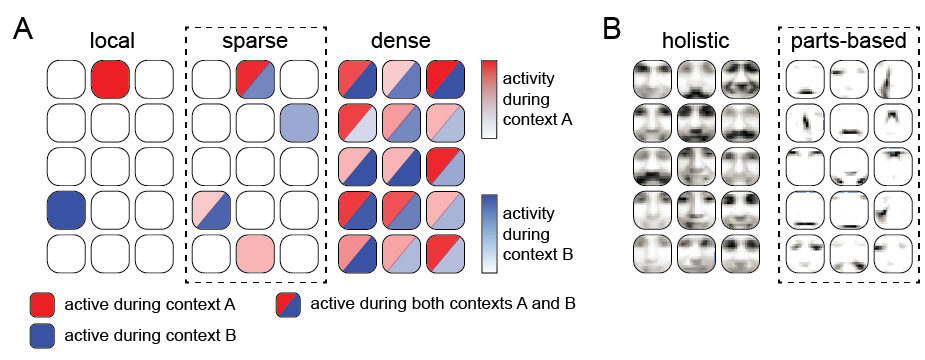
\includegraphics[width=\textwidth]{fig-rev1-sparse}
    \caption{\Acf{NSC} promotes population codes that are both sparse and parts-based.
    \textbf{\emph{A}},
    	   Hypothetical activity in a population of neurons
           during presentation of two different external stimuli (`contexts').
           A sparse code is a trade-off between a local code
           (where a context is represented by the activity of a single neuron,
           and different contexts are represented by different neurons), and a
           dense code (where all neurons are active and their combined activity is
           used to encode each context).
           Dense codes possess great memory capacity, but suffer from cross talk
           among neurons, whereas local codes do not suffer from interference
           but also have no capacity for generalization
           (adapted from \cite{SpanneJorntell2015}).
     \textbf{\emph{B}},
           In a holistic representation of faces, 
           individual neurons in the population
           respond themselves to faces as a whole \cite{TanakaFarah1993},
           whereas in a parts-based representation
           individual neurons explicitly encode individual face components
           \cite{Palmer1977},
           such as the eyes, nose, and mouth
           (adapted from \cite{LeeSeung1999}).}
	\label{fig:sparse-parts}
\end{figure}


Another approach is to reduce the number of
variables required to represent a particular stimulus space;
a process known as
\textbf{dimensionality reduction}.
Dimensionality reduction methods have proved useful in elucidating neural mechanisms
that depend on how the responses of multiple neurons covary,
including odor discrimination in the olfactory system \cite{Broome2006,Koulakov2011},
the selection and integration of sensory inputs 
in the prefrontal cortex \cite{Mante2013},
and the ability of premotor cortex 
to prepare movements without executing them \cite{Kaufman2014}.

In brain areas far removed from sensory input,
neurons typically encode several behaviorally relevant parameters
simultaneously \cite{Rigotti2013,Park2014,PaganRust2014,PougetSejnowski1997},
allowing for multifaceted representations of high-dimensional stimulus spaces.
For example, a population of neurons tasked with encoding human faces
might opt to represent each individual face as a combination of a set of
standard faces (Fig.~\ref{fig:sparse-parts}B, left column).
In such a \textbf{holistic representation} of faces \cite{TanakaFarah1993},
each individual neuron would itself respond to a face as a whole
(i.e., a face `template')
without explicitly representing individual face components,
and an arbitrary face could be represented by 
combining different face templates
(e.g., by adding 10\% of template 1 to 20\% of template 2
and subtracting 30\% of template 3).
On the other hand, faces can also be represented as a combination
of individual face components, such as eyes, noses, and mouth,
in what is known as a \textbf{parts-based representation}
(Fig.~\ref{fig:sparse-parts}B, right column) \cite{Palmer1977}.
Both approaches allow for representing arbitrary faces as a combination of
neural activity, but have drastically different consequences on the
set of stimulus features each neuron responds to.
Although visual information from the eyes, nose, and mouth would of course be
included in a holistic face representation,
that information would not be explicitly represented as structural units
in their own right \cite{TanakaFarah1993}.
Linear combinations of holistic components often involve complex cancellations
between positive and negative contributions,
and thus lack the intuitive meaning of adding parts to form a whole.
In contrast, a parts-based representation allows for only nonsubtractive
combinations of stimulus features \cite{Palmer1977}.
Although the relevant stimulus dimensions are often not known \emph{a priori},
several sophisticated mathematical techniques exist that
allow us to discover these representations directly from experimental data
\cite{Brunton2016,CunninghamYu2014,PillowSimoncelli2006,Sharpee2014,Gao2017}.

In this article, we demonstrate that a variety of neuronal responses
can be understood as an emergent property of efficient population coding
based on dimensionality reduction and sparse coding.
Specifically, we review computational evidence
from data analyses and computer simulations arguing that \ac{NSC}, 
a combination of \textbf{\ac{NMF}}
\cite{PaateroTapper1994,LeeSeung1999} 
and sparse coding,
can generate sparse and parts-based embeddings of
high-dimensional stimulus spaces
that resemble neuronal population responses in a 
wide variety of brain regions.
This introduces the possibility that \ac{NSC} might
be a general principle to which many neuronal computations adhere.
Furthermore, \ac{NSC} might provide a useful theoretical framework under which
to understand the often complex and nonintuitive response properties of neurons
in brain areas far removed from sensory input.

\section*{Nonnegative sparse coding (NSC) as a modern variant of the efficient coding hypothesis}

\subsection*{Efficient coding}

The fundamental principle of \textbf{efficient coding}
is that a sensory system is
adjusted to the specific statistics of the natural environment from which
it encodes and transmits information
\cite{Barlow1961,Attneave1954,Linsker1990,LouieGlimcher2012}.
\revise{Efficiency, in this context, is an information-theoretic term 
that should not be confused with `minimizing energy expenditure'.
Instead, a sensory pathway is treated as a noisy communication channel, where 
the goal is to maximize the rate at which information can be reliably transmitted
by minimizing the redundancy between representational units.}

Early theories of efficient coding
\cite{Barlow1961,Attneave1954}
were developed based on the visual system.
Attneave \cite{Attneave1954} pointed out that there is a significant
degree of redundancy in natural visual images due to correlations in both
the spatial and temporal domains
(for a recent review, see \cite{SimoncelliOlshausen2001}).
For example, the luminance values of a pair of pixels
separated by a fixed distance in a natural image
are likely to be highly correlated
(Fig.~\ref{fig:ech}A).
These statistical regularities constrain the images a visual system
is likely to encounter to a tiny fraction of the set of all
possible images.
It was therefore argued that the visual system should not
waste resources on processing arbitrary images,
but instead use statistical knowledge
about its environment to represent the relevant input space 
as economically as possible.


\begin{figure}[h]
	\centering
% 	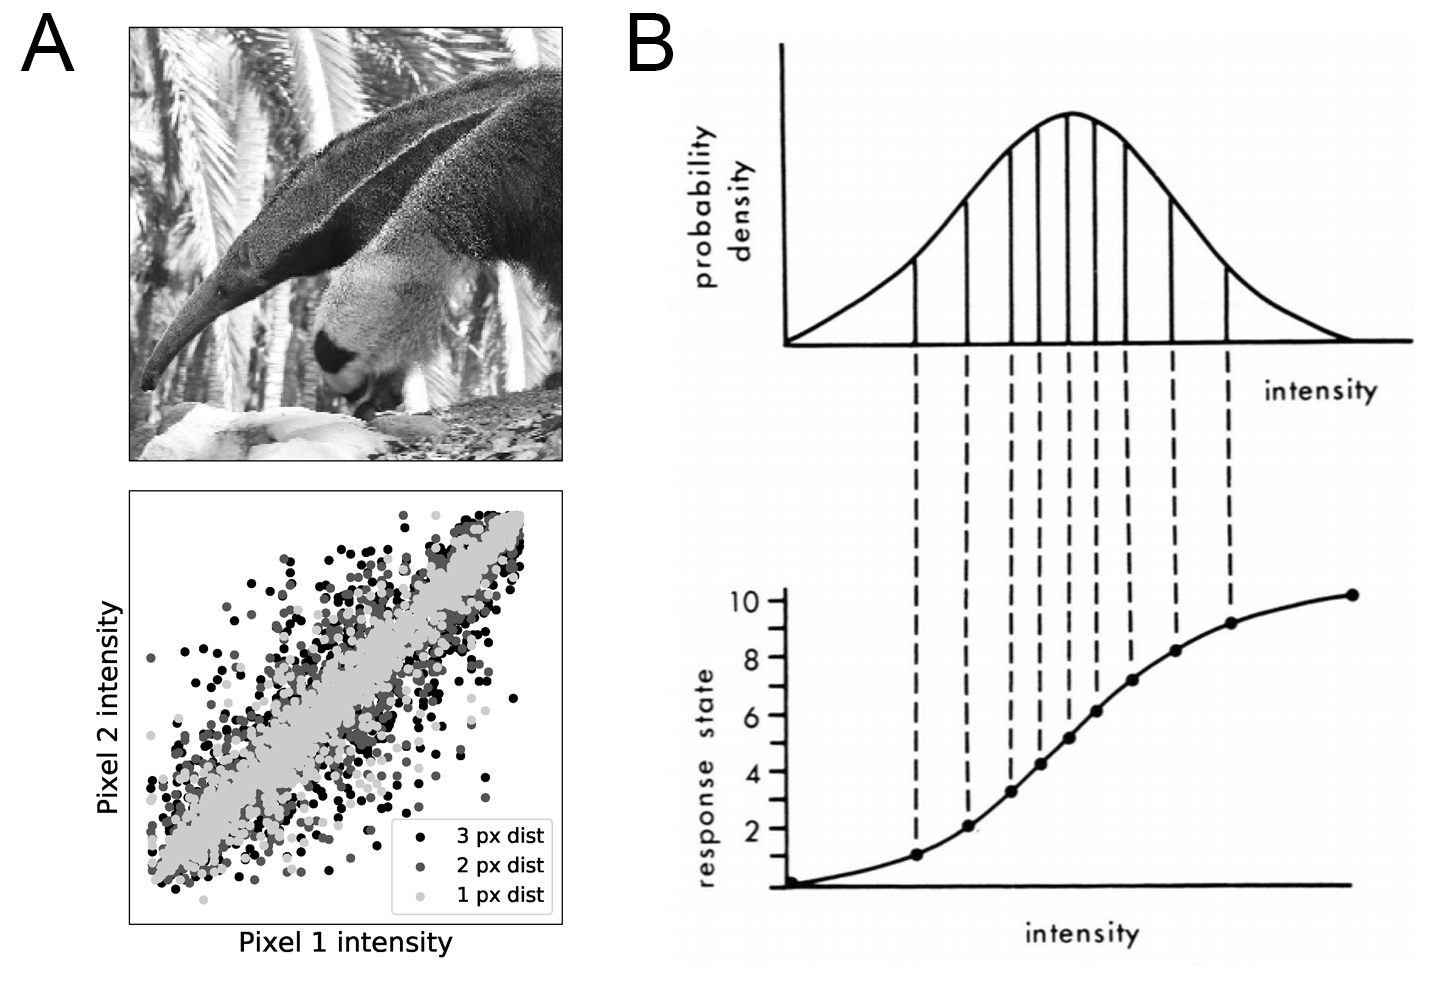
\includegraphics[width=\textwidth]{fig-rev2-ech}
    \caption{Efficient coding hypothesis.
    \textbf{\emph{A}},
         Sensory stimuli in the environment, such as an image of \revise{an anteater},
         display significant statistical structure. For example, the luminance
         value of nearby pixels in the image are significantly correlated,
         an effect that exists even for nonadjacent pixels \revise{(inspired by \cite{LouieGlimcher2012})}.
         Neural systems can improve their coding efficiency by accounting
         for and reducing such information redundancy.
     \textbf{\emph{B}},
         For a given distribution of sensory characteristics in the world \revise{(top)},
         \revise{a neuron's information capacity is maximized 
         when all response levels are used with equal frequency
         (reprinted from \cite{Laughlin1981} under CC-NC-ND 3.0).
         Intervals between each response level encompasses an equal area
         under the intensity distribution, so each state is used with
         equal frequency.}
    }
	\label{fig:ech}
\end{figure}


Extending this idea to the neural level,
Barlow \cite{Barlow1961} proposed that
the goal of early neurons in sensory processing is to remove
the redundancy in the input stimuli.
These ideas were shaped by two
fundamental empirical observations
about early visual cortex:
1) a neuron's \ac{RF} resembled a decomposition of the visual
stimulus into a series of local, largely independent feature components
(e.g., a 2-D Gabor function is basically a local approximation of the
directional spatial derivative of an image),
and 2) any individual neuron responded only sparsely to a small subset of
stimulus features (e.g., orientation or color at a particular spatial location).
Thus a neuron's \ac{RF} could be understood as a
sparse, low-dimensional embedding of high-dimensional input stimuli
\cite{Barbieri2015}.
\revise{However, there is the possibility that sparsity results from a limited stimulus set as we discuss in the ``Model limitations'' section.}

At the level of single neurons, efficient coding requires
that a neuron's input-output function be adjusted so that all
activity levels are used equally in response to a specific
stimulus distribution \cite{Simoncelli2003} (see Fig.~\ref{fig:ech}B).
If the input-output function sensitivity is too low,
high levels of the stimulus feature will be indistinguishable
as the response function saturates; if the sensitivity is set too high,
low levels of the stimulus feature cannot drive responses 
\cite{Laughlin1981}.

At the level of neuronal populations,
neural responses should be both \emph{decorrelated}
(i.e., independent from one another)
and \emph{sparse}
(i.e., involve only a small fraction of neurons in the population)
\cite{LouieGlimcher2012}.


\subsection*{Sparse coding}

Taking these ideas a step further,
Olshausen and Field \cite{OlshausenField1996b} 
noted that natural images contain statistical
dependencies beyond linear pairwise correlations among image pixels,
and argued that these higher-order correlations should be taken into
account when developing an efficient code.
Their goal was thus to find a linear coding strategy
capable of reducing these higher-order forms of redundancy.

\emph{Linear sparse coding} is one such strategy,
where monochromatic images $I(x,y)$
are described in terms of a linear superposition of
a number of \textbf{basis functions},
$w_b(x,y)$:
\begin{equation}
I(x,y) = \sum^B_{b=1} w_b(x,y) h_b,
\label{eqn:sparse-coding}
\end{equation}
where $h_b$ are stochastic coefficients that are different for each image
\cite{OlshausenField1996,Hyvarinen2001}.
Learning a sparse code for images thus involved determining
the values of both $w_b(x,y)$ and $h_b$ for all $b$ and $(x,y)$,
given a sufficient number of observation of images,
under the constraint that $h_b$ be sparse.
In this context, $h_b$ was considered sparse if it took very small
or very large (absolute) values more often than a Gaussian random
variable would \cite{Hyvarinen2001}.
This sparsity constraint allowed for basis functions that were not
needed to describe a given image structure to be weeded out.

\revise{Sparsity, in this context, is an information-theoretic concept
related to how efficiently and completely information is encoded with
the basis functions described above.
Please note that this is different from empirical observations
of brain areas being `sparsely' activated; that is,
sparse population activity does not necessarily imply that a brain area
implements a sparse coding scheme.
This confusion is fueled in part by the wide variety of definitions of sparsity
used in the literature\cite{SpanneJorntell2015,BarthPoulet2012}.}

When Olshausen and Field applied linear sparse coding 
to natural images,
they found that the emerging basis functions 
were qualitatively similar in form
to \acp{RF} of simple cells in \ac{V1} 
\cite{OlshausenField1996,OlshausenField1997},
thus giving empirically observed \acp{RF} 
an information-theoretic explanation.
In this context, $h_b$ in Eq.~\ref{eqn:sparse-coding} above
corresponded to the (signed) activation value of a particular \ac{V1}
neuron, and $w_b(x,y)$ were the connection weights
(or \emph{synaptic weights} in an artificial neural network)
that were closely related to that neuron's \ac{RF}.
Olshausen and Field went on to show that 
the set of basis functions that best described \ac{V1} \acp{RF} 
was greater in number than the effective
dimensionality of the input
(\revise{which they termed} an \emph{overcomplete} basis set) 
\cite{OlshausenField1997}.
\revise{It is worth noting that sparse coding with an overcomplete basis set
is typically associated with an anatomical fan-out motif,
such as expanding 1 million optic nerve fibers 
into more than 100 million \ac{V1} neurons,
or from a small number of mossy fibers to a 100-fold larger number of
granule cells in the cerebellum.}

However, as pointed out by Hoyer \cite{Hoyer2003}, 
linear sparse coding falls short of providing a literal interpretation
for \ac{V1} simple-cell behavior for two reasons:
1) every neuron could be either positively or negatively active, and
2) the input to the neural network was typically double-signed,
whereas \ac{V1} neurons receive visual input from the \ac{LGN} 
in the form of separated, nonnegative ON and OFF channels.

In order to transform Olshausen and Field's sparse coding
from a relatively abstract model of image representation 
into a biologically plausible model of early visual cortex processing,
Hoyer \cite{Hoyer2002,Hoyer2003} thus proposed to enforce
both input signal and neuronal activation to be nonnegative.
This seemingly simple change had remarkable consequences 
on the quality of the sensory representation:
Whereas elementary image features in the standard sparse coding model
could `cancel each other out' through subtractive interactions,
enforcing nonnegativity ensured that features combined additively,
much like the intuitive notion of combining parts to form a whole.
The resulting parts-based representations resembled \acp{RF} in \ac{V1} 
much more closely than other holistic representations.
These considerations led to the formulation of nonnegative sparse coding (\ac{NSC}) in its current form.


\subsection*{Nonnegative sparse coding (NSC)}

As a special case of linear sparse coding,
\ac{NSC} shares the same goal of accurately describing observed data
as a superposition of a set of sparsely activated basis functions.
However, \ac{NSC} additionally requires 
all basis functions and activation values
(i.e., $w_b(x,y)$ and $h_b$ in Eq.~\ref{eqn:sparse-coding})
to be nonnegative.

Consider $S$ observed stimuli or data samples,
each comprised of $F$ observed feature values,
such as a collection of $S$ images $I(x,y)_s$ ($s \in [1, \ldots, S]$)
from the example above,
each consisting of $F$ different grayscale values.
If we arrange the observed feature values of the $s$-th observation into
a vector $\vec{v}_s$ (i.e., by flattening each observed image),
and if we arrange all vectors into the columns 
of a $F \times S$ data matrix \textbf{V},
then linear decompositions describe these data as:
\begin{equation}
\mathbf{V} \approx \mathbf{WH},
\label{eqn:linear-decomposition}
\end{equation}
where \textbf{W} is a $F \times B$ matrix that contains as its columns
the $B$ basis functions of the decomposition
(i.e., the $b$-th column of \textbf{W} corresponding to 
$w_b(x,y)$ $\forall x,y$ in Eq.~\ref{eqn:sparse-coding}),
and \textbf{H} is a $B \times S$ matrix containing
as its columns the activation values 
of each basis function for a particular input stimulus
(i.e., the $b$-th column of \textbf{H} corresponding to 
$h_b$ $\forall b$ in Eq.~\ref{eqn:sparse-coding}).
The difference between \textbf{V} and \textbf{WH} is termed
the \emph{reconstruction error}.

The goal of \ac{NSC} is then to find a linear decomposition of \textbf{V}
that minimizes the reconstruction error,
while guaranteeing that \textbf{H} is sparse.
This can be achieved by minimizing the following cost function
\cite{Hoyer2002}:
\begin{equation}
\min_{\mathbf{W}, \mathbf{H}} \frac{1}{2} ||\mathbf{V} -\mathbf{WH}||^2 + \lambda \sum_{ij} f(\mathbf{H}_{ij}),
\label{eqn:nsc-cost-function}
\end{equation}
subject to the constraints
$\forall ij: \mathbf{W}_{ij} \geq 0$, $\mathbf{H}_{ij} \geq 0$, and
$||\vec{w}_i|| = 1$, where $\vec{w}_i$ denotes the 
$i$-th column of \textbf{W}.
Here, the left-hand term describes the reconstruction error,
whereas the right-hand term describes the sparsity of the decomposition.
The trade-off between accurate reconstruction and sparsity
is controlled by the parameter $\lambda$ ($\lambda \geq 0$), whereas
the form of $f$ defines how sparsity is measured
(a typical choice is the L1 norm on \textbf{H}).
\revise{\Ac{NSC} explicitly discourages statistically inefficient representations,
because strongly accounting for a rare observation 
at the expense of ignoring a more common one stimulus component
would result in an increased reconstruction error.}

In the case of $\lambda = 0$, Eq.~\ref{eqn:nsc-cost-function}
reduces to the squared-error version of \textbf{\ac{NMF}}.
Although \ac{NMF} enforces all elements of \textbf{W} and \textbf{H}
to be nonnegative,
the resulting decomposition might not be sparse,
depending on the number of basis functions $B$.
In order to emphasize decompositions where \textbf{H} is sparse,
Eq.~\ref{eqn:nsc-cost-function} should be minimized 
with $\lambda > 0$ \cite{Hoyer2002}.

Another open parameter is the number of basis functions, $B$, 
which controls the predictive power of the model,
and must be determined empirically.
With a small number of basis functions,
\ac{NSC} is unlikely to achieve a low reconstruction error
be it in familiar contexts (training data) or in novel contexts
(held-out test data).
In this case, the error depends on the systematic bias of the model,
and the model is said to \emph{underfit} the data
(left-hand side of Fig.~\ref{fig:nsc-bias-variance-dilemma}).
With increased model complexity,
the model can learn subtle differences 
between different contexts with high accuracy,
leading to a reduced bias (training) error.
However, with increased complexity, the model is more likely to learn
patterns between training contexts that arise either from underlying noise
or from spurious correlations. As a result,
the model will respond according to
these learned patterns when a novel context is presented
(rather than according to the underlying actual relationships), 
in which case the model is said to \emph{overfit} the data
(right-hand side of Fig.~\ref{fig:nsc-bias-variance-dilemma}).
Hence, the goal of a successful model is to find the ideal compromise
in the bias-variance error trade-off \cite{Beyeler2017}
(labeled `best model' in Fig.~\ref{fig:nsc-bias-variance-dilemma}).

\begin{figure}[h]
	\centering
% 	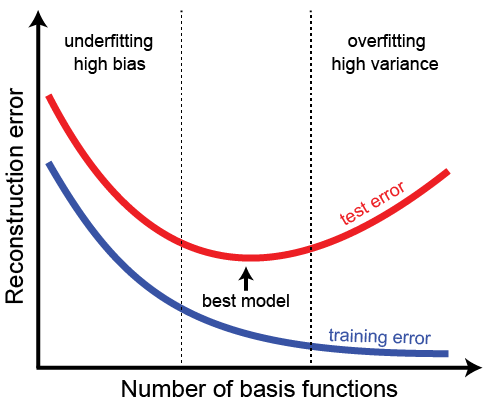
\includegraphics[width=0.6\textwidth]{fig-rev1-bias-variance}
    \caption{The bias-variance dilemma.
    With increased model complexity 
    (i.e., with an increased number of basis functions), 
    the reconstruction error on a set
    of familiar (training) data typically decreases until it reaches zero.
    In contrast, the reconstruction error on a set of unfamiliar, held-out
    (test) data typically goes through a minimum as a function of model complexity.
    A successful model chooses the number of basis functions such that the
    generalization (test) error is minimized (labeled `best model`).}
	\label{fig:nsc-bias-variance-dilemma}
\end{figure}

Analogously to \cite{OlshausenField1996,OlshausenField1997},
the basis functions obtained in \ac{NSC} can be interpreted as
the connection weights of a population of simulated neurons
in an artificial neural network.
In other words, under \ac{NSC} the number of basis functions $B$ 
corresponds to the number of output neurons, and the
response of the $b$-th model output neuron
($b \in [1, ..., B]$)
to a particular input stimulus $s$, termed $r_{bs}$,
can be computed by feeding the dot product of
that neuron's connection weights
(i.e., the $b$-th column in $\mathbf{W}$, $\vec{w}_b$)
and a data vector
(i.e., the $s$-th column in \textbf{V}, $\vec{v}_s$)
to an activation function $\Theta$:
\begin{equation}
r_{bs} = \Theta(\vec{w}_b \cdot \vec{v}_s),
\label{eqn:nsc-model-response}
\end{equation}
where $\cdot$ denotes the dot product.
For example, the linear response of a model neuron
can be calculated by setting $\Theta$ to the identity function $\Theta(x)=x$.
Note that the response of the model neuron to different stimuli 
$s \in [1, \ldots, S]$
involves different columns of \textbf{V},
but always relies on $\vec{w}_b$.

Inhibitory connections can be modeled in the same fashion,
by interpreting inhibitory connection weights
as nonnegative synaptic conductances.
\revise{For example, Hoyer \cite{Hoyer2003} used \ac{NSC} to model \ac{V1} neurons
as receiving input from both excitatory ON and inhibitory OFF cells in the \ac{LGN}.
Using pre-whitened natural images, Hoyer sampled $12 \times 12$ pixel patches from
the images, and then separated positive and negative values into separate channels.
Each image patch was thus represented by a $2 \times 12 \times 12 = 288$ dimensional vector,
each element of which mimicked the activity of an ON or OFF cell
in response to the image patch.
These vectors were then arranged into the columns of \textbf{V}.}
This procedure not only preserved the parts-based quality of the encoding,
but also allowed for more complicated connection types to be modeled.
However, it is interesting to note that a more recent study has argued
that the nonnegativity constraint on the
connection weights might not be necessary 
to preserve the parts-based quality of the encoding (see \cite{Liu2017}).

Thus, we can utilize \textbf{W} 
(which must remain fixed once learned)
and Eq.~\ref{eqn:nsc-model-response}
to simulate a model neuron's response to arbitrary input stimuli
by replacing the column in \textbf{V} with new input.
This allows us to investigate the response properties 
of individual model neurons
much in the same way that experimental neuroscientists 
study biological neurons.
This is important because it means that \ac{NSC} can be used to 
model neural activity in the brain, 
and the resulting activity patterns generated by \ac{NSC}
can be compared to and evaluated against experimental findings. 


\section*{Empirical evidence for nonnegative sparse coding in the brain}

An influential paper by Lee and Seung \cite{LeeSeung1999}
found that applying \ac{NMF} to a database of face images
yielded sparse, localized features that resembled parts of a face
\revise{(Fig.~\ref{fig:NMF|reconstruction}A)}.
In their case, \ac{NMF} acted on a
$F \times S$ data matrix \textbf{V},
whose rows corresponded to distinct features of the input 
(e.g., $F$ different pixels of an image)
and whose columns corresponded to different stimuli or 
observations of those features
(e.g., $S$ different images).
\ac{NMF} was used to decompose the matrix into two reduced-rank matrices
(Fig.~\ref{fig:NMF|reconstruction}, \revise{inset})
whose linear combination could be weighted such that the product of \textbf{W} and \textbf{H} provided an accurate reconstruction of \textbf{V}
\revise{(see Eq.~\ref{eqn:linear-decomposition}).}

A particular image, in this case encoded by $F = 19 \times 19 = 361$ pixels
could be accurately represented by a linear combination of 
a small number ($B = 49$) of encoding variables or `basis images'
(Fig.~\ref{fig:NMF|reconstruction}\revise{A}).
Such a representation is reminiscent to neural processing in \ac{IT},
an area in the ventral visual `what' stream
involved in encoding high-level object identity
\cite{BrincatConnor2004,Majaj2015},
where images of whole faces can be linearly reconstructed
using responses of approximately $200$ neurons
that each respond to a certain set of physical facial features
\cite{ChangTsao2017}.

\begin{figure}[ht]
	\centering
% 	\includegraphics[width=\textwidth]{fig4}
    \caption{\revise{Sparse and parts-based representations recovered by \ac{NMF}
             resemble receptive fields across brain regions.
             \Ac{NMF} (inset) can reconstruct a} data matrix \textbf{V}
             ($F$ features x $S$ stimuli)
             from two reduced-rank matrices \textbf{W}
             (containing $B$ basis functions) and \textbf{H}
             (containing the hidden coefficients of the decomposition).
             Any individual input stimulus (i.e., column in \textbf{V}, \revise{red})
             can be reconstructed from a linear combination
             \revise{(i.e., column in \textbf{H}, blue)}
             of a set of basis functions (i.e., all columns in \textbf{W}, 
             \revise{green}).
         \textbf{\emph{A}},
             A facial image can be reconstructed from a sparse activation
             of simulated \acs{IT} neurons that
             preferentially respond to parts of faces
             (adapted from \cite{LeeSeung1999}).
         \textbf{\emph{B}},
             An optic flow field can be reconstructed from a sparse
             activation of model \acs{MSTd} neurons that prefer various
             directions of 3D self-translation and self-rotation
             (adapted from \cite{Beyeler2016}).
         \textbf{\emph{C}},
             A rat's 2D allocentric position and route-based direction of
             motion can be reconstructed from a sparse activation of
             model \acs{RSC} neurons that prefer an intricate combination of
             linear velocity (LV), angular velocity (AV), head direction (HD)
             and 2D position (P).
             For the sake of clarity, only the 4 most contributing hidden
             coefficients (out of 30) are shown.}
	\label{fig:NMF|reconstruction}
\end{figure}


\revise{Interestingly}, such a parts-based representation is not specific to
information processing in \ac{IT};
the same principle can be extended to other areas of the visual system,
such as the \ac{MSTd},
which is part of the visual motion pathway \cite{Beyeler2016}.
Neurons in \ac{MSTd} respond to relatively large and complex patterns
of retinal motion (`optic flow'),
owing to input from direction and speed selective neurons in the \ac{MT}
(for a recent review, see \cite{Orban2007}).
Although \ac{MSTd} had long been suspected to be involved in the
analysis of self-motion,
the complexity of neuronal response properties has made it difficult
to experimentally investigate how neurons in \ac{MSTd}
might perform this function.
However, when \revise{our group} 
applied \ac{NMF} to 
\revise{simulated neural activity patterns whose statistical properties
resembled that of experimentally recorded \ac{MT} neurons} 
\cite{Beyeler2016},
\revise{we} found a sparse, parts-based representation of retinal flow
(Fig.~\ref{fig:NMF|reconstruction}\revise{B})
similar to the parts-based representation of faces
encountered by Lee and Seung \cite{LeeSeung1999}.
The resulting `basis flow fields' showed a remarkable resemblance to receptive fields
of \ac{MSTd} neurons, as they \revise{responded to}
an intricate mixture of
3D translational and rotational flow components
in a subset of the visual field.
As a result, any flow field possibly to be encountered 
during self-movement through a 3D environment
could be represented by only $B = 64$ simulated \ac{MSTd} neurons,
as compared to $F = 9,000$ simulated \ac{MT} input neurons.
This led to an sparse \revise{and parts-based} population code,
where any given stimulus could be represented
by only a small number of simulated \ac{MSTd} neurons
\cite{Beyeler2016}.

Analogously, \ac{NSC} can explain response properties
of neurons outside the visual system, 
such as in the \ac{RSC}, an area in the posterior cingulate region
important for navigation and spatial memory \cite{Miller2014,Nelson2015,VannAggleton2009}.
Neurons in the \ac{RSC} conjunctively encode multiple variables related to the environment and one's position and movement within it
\revise{(e.g., position, head direction, linear velocity, and angular velocity)},
allowing the representation of spatial features of the environment 
with respect to multiple reference frames \cite{AlexanderNitz2015}.
\revise{When our group applied \ac{NMF} to neurophysiological data from
\ac{RSC} neurons while rats ran back and forth on a W-shaped track
(for experimental details, see Supplementary Materials),
we again found a sparse and parts-based representation for behaviorally
relevant variables such as the animal's position, head direction, 
and movement direction (Fig.~\ref{fig:NMF|reconstruction}C).
Interestingly, model \ac{RSC} neurons encoded these variables with respect
to multiple frames of reference
(e.g., head direction: \textbf{allocentric reference frame},
linear velocity: \textbf{route-based reference frame}).
Once again, the dimensionality of the stimulus space was drastically reduced
from $F = 417$ input neurons to a set of $B = 30$ model \ac{RSC} neurons.}

\revise{Due to its roots in efficient-coding theories of natural image processing,
there is a large body of research highlighting the role of \ac{NSC} in
visual cortex function
(e.g., \cite{Barlow1961,OlshausenField1996,Hoyer2003,BenHamed2003}).}
Although there seems to be a consensus that 
information-theoretic explanations are relevant 
when investigating the early visual system,
higher-order brain areas are often considered to be specialized for
performing tasks
(e.g., recognizing objects, making decisions, navigating an environment),
rather than the efficient encoding of information.

\revise{However, more recently, 
\ac{NSC}-like computational models have found application outside visual cortex,
where they have started to provide compelling evidence that a wide variety of
neuronal response properties can be understood as an epiphenomenon
of efficient population coding based on dimensionality reduction.
Examples include elucidating the dimensions along which perceptual space
is organized in the olfactory system
\cite{MorenoBoteDrugowitsch2015,Castro2013},
the coordination of movement in the cortico-basal ganglia-thalamo-cortical loop
\cite{BarGad2000,BarGad2003_Review},
and the combined representation of allocentric and route-based 
spatial navigation cues
in retrosplenial cortex \cite{Rounds2018}.}
\revise{The success of these models suggests that \ac{NSC}}
might apply elsewhere in the brain, 
\revise{thus warranting further investigation.}
In fact, sparse (and potentially parts-based) representations have been observed
in \revise{a wide variety of brain areas}
(see Table~\ref{table:listEvidence}).
This introduces the \revise{intriguing} possibility that \ac{NSC} might
be a general principle to which \revise{many} neuronal computations adhere.
\revise{In the future, \ac{NSC} might provide a useful theoretical framework
under which to understand the often complex and nonintuitive response properties
of neurons in brain areas far removed from sensory inputs,
including the selection and integration of various task-related variables
in prefrontal cortex
\cite{Mante2013}
and the ability of premotor cortex to prepare movements without executing them
\cite{Kaufman2014}.}



\begin{table}[ht]
\begin{adjustwidth}{-2.25in}{0in}
	\centering
	\caption{Nonnegative sparse coding in the brain.
    We list a group of brain regions for which there is experimental evidence of certain features associated with NSC (`X': evidence exists, `?': has yet to be investigated).
   For each brain region, the left-hand side of the table lists experimental evidence for sparse \revise{population codes} and/or parts-based representations, whereas the right-hand side lists computational support that \revise{\ac{NSC}-like models} can describe receptive fields or response properties within that region.}
    \def\arraystretch{1.1}
    {\setlength{\tabcolsep}{1em}
    \begin{tabular}{r|rrr|rr}
	\revise{\textbf{Brain}} & \textbf{Sparse} &  \textbf{Parts-} & \textbf{Experimental} & \textbf{Modeled} & \textbf{Computational} \\
	\textbf{Area} & \revise{\textbf{code}} & \textbf{based} & \textbf{evidence} & \textbf{by NSC} & \textbf{ support} \\ \hline
    Retina & X & X & \cite{Onken2016,Liu2017} & X & \cite{Onken2016,Liu2017} \\
    \revise{Visual cortex} & X & X & \pbox{5cm}{\cite{OlshausenField1996,HoyerHyvarinen2002,vanHateren1998,Wachsmuth1994,FreiwaldTsao2010,ChangTsao2017,BenHamed2003}} & X & \pbox{5cm}{\cite{OlshausenField1996,Hoyer2003,Carlson2013,Hyvarinen2001,LeeSeung1999,Hosoda2009,Beyeler2016}} \\
    Auditory cortex & X & \revise{X} & \revise{\cite{Hromadka2008,rokem2006,bendor2008,Leaver2010,Terashima2013,SmithLewicki2006}} & \revise{X} & \revise{\cite{Martinez2015,David2007}} \\
 	Olfactory cortex & X & \revise{X} & \cite{Koulakov2011,poo2009,rinberg2006,Broome2006,Castro2013} & \revise{X} & \revise{\cite{MorenoBoteDrugowitsch2015,Castro2013}}  \\
 	\revise{Somatosensory} cortex & X  & \revise{X} & 			   \revise{\cite{Jadhav2009,oconnor2010,Crochet2011,Ramirez2014,penfield1937,hari1993,petersen2007}} & \revise{X} & \revise{\cite{WhitewayButts2017,Hafner2004}}  \\
    \revise{Parietal cortex} & \revise{?} & \revise{X} & \revise{\cite{Poggio1990,PougetSejnowski1997,andersen1997multimodal,PougetSnyder2000,louie2015adaptive}} & \revise{?} & \revise{?}  \\
    Retrosplenial cortex & \revise{?} & X & \revise{\cite{AlexanderNitz2015,vedder2016,mao2017}} & X & \cite{Rounds2018} \\
    \revise{Prefrontal cortex} & \revise{?} & \revise{?} & \revise{\cite{Mante2013,Rigotti2013,Fujisawa2008,Wei2015}} & \revise{?} & \revise{?}  \\    
    Motor cortex & \revise{?} & \revise{?} & \revise{\cite{Beloozerova2003,penfield1937,GrazianoAflalo2007,Brecht2004}}
    & ? & \revise{?} \\
    Hippocampus & \revise{X} & \revise{?} & \revise{\cite{ThompsonBest1989,Bakker2008,myers2011pattern,rolls2013,Wixted2014,Poli2017}} & \revise{?} & \revise{?} \\        
    Basal ganglia & X & ? & \cite{BarGad2003_Review,Turner2000,schwab2015} & X & \pbox{5cm}{\cite{BarGad2000,BarGad2003_Review}} \\  
	\end{tabular}}
    \label{table:listEvidence}
\end{adjustwidth}
\end{table}

\revise{In the following subsections,
we review existing experimental evidence
for sparse and parts-based representations 
in various brain areas highlighted in Table~\ref{table:listEvidence}.
Where available, we highlight \ac{NSC}-like computational models
that  successfully explain response properties of individual neurons
or have been instrumental in elucidating the dynamics at the population level.}


\subsection*{Understanding neuronal response properties within the framework of NSC}

\mikeNote{This first subsection is so basic and integral to understanding how NMF maps to neurons that it would almost make sense to move it to subsection ``Nonnegative sparse coding'' in the background section. We would probably add a figure there that shows the NMF schematic V=WH and Fig.4 panel A, so that the reader immediately understands the processing pipeline of how to go from W in NMF to $r_bs$.}

By interpreting the elements of \ac{NMF}'s
matrix \textbf{W} as the synaptic weights of model output neurons,
\ac{NSC} allows for the computation of neuronal response properties
with
methods similar to the ones employed by experimental researchers to understand biological neurons,
and by theoretical neuroscientists to understand computational models. This is important because it means that NSC can be used to model neural activity in the brain, and the resulting activity patterns generated by NSC can be compared to and evaluated against experimental findings. 

In \ac{NSC}, the number of basis functions $B$ corresponds to the number of output neurons. The response of the $b$-th model output neuron
($b \in [1, ..., B]$)
to a particular input stimulus $s$, $r_{bs}$,
can be computed by feeding the dot product of the neuron's presynaptic connections
(i.e., the $s$-th column in \textbf{V})
and the corresponding synaptic weights
(i.e., the $b$-th column in $\mathbf{W}$)
to an activation function $\Theta$
(Fig.~\ref{fig:NMF|neuronalresponse}A).
For example, the linear response of a model neuron
can be calculated by setting $\Theta$ to the identity function $\Theta(x)=x$.
Note that the response of the model neuron to different stimuli 
$s \in 1, \ldots, S$
involves different columns of \textbf{V},
but always relies on the same weight matrix \textbf{W}.
Thus, we can utilize \textbf{W}
(which must remain fixed once learned with \ac{NMF})
to simulate a model neuron's response to arbitrary input stimuli
by replacing the column in \textbf{V} with new input.
This allows us to investigate the response properties of individual model neurons
much in the same way that experimental neuroscientists study biological neurons.

\begin{figure}[h]
	\centering
	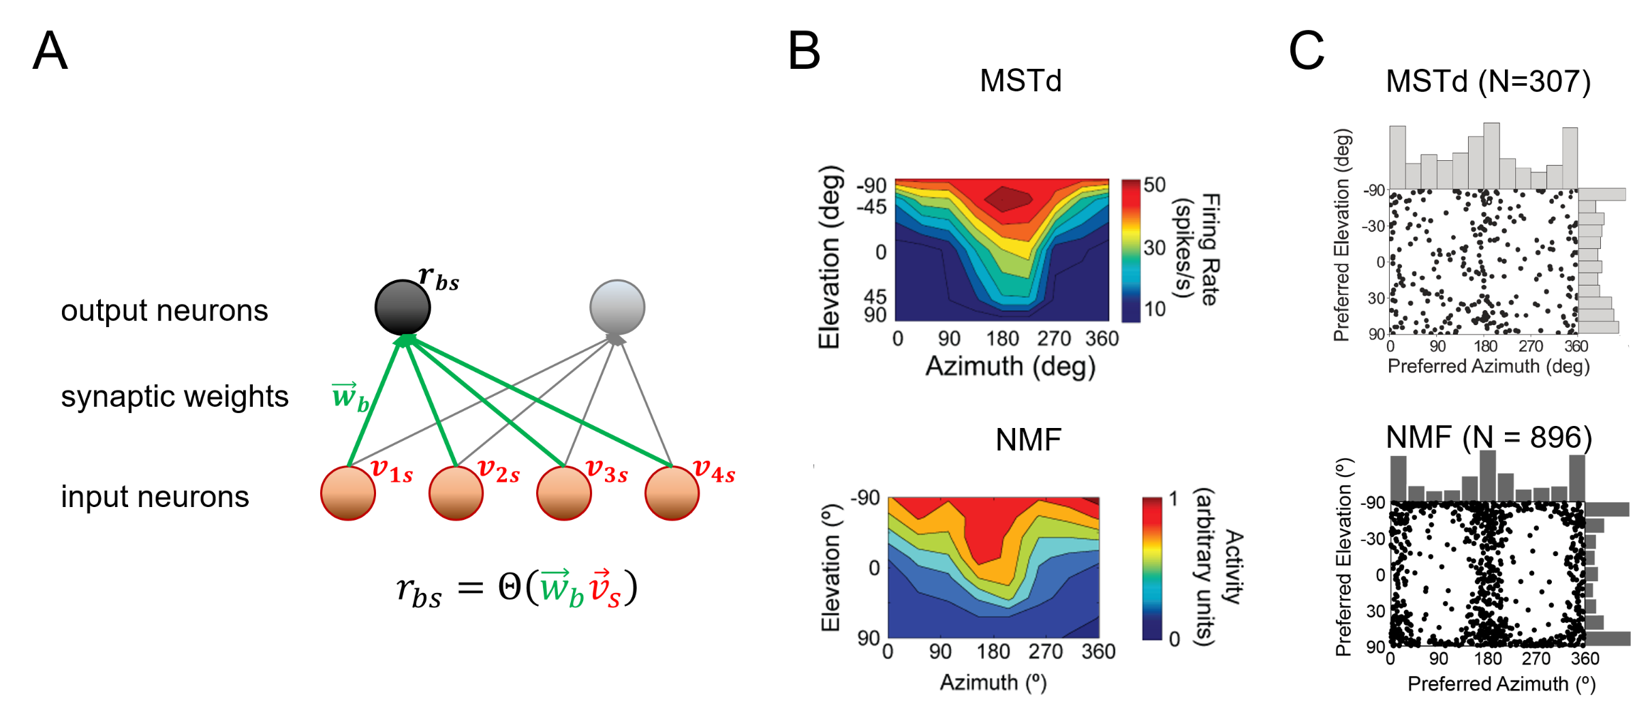
\includegraphics[width=\textwidth]{fig-rev1-responses}
    \caption{\ac{NSC} can predict response properties of biological neurons.
    A) $r_{bs}$ is the response of the $b$-th model output neuron
       to the $s$-th stimulus. $r_{bs}$
       can be calculated from the activity of all
       input neurons (i.e., column $s$ in \textbf{V}), the
       corresponding synaptic weights (i.e., column $b$ in
       $\mathbf{W}$), and a neuronal activation function $\Theta$.
    B) Example of 3D heading tuning for a neuron in macaque
       \ac{MSTd} (top, reprinted from \cite{Takahashi2007}) and a
       simulated neuron (bottom,
       based on the linear response using $\Theta(x)=x$,
       reprinted from \cite{Beyeler2016}).
       Color contour maps show the mean firing rate or model
       activation as a function of azimuth and elevation angles
       of the self-movement direction in 3D.
    C) Classifying simulated akin to biological neuronal responses
       yields distributions of 3D heading preferences akin to 
       macaque \ac{MSTd} (top, reprinted from \cite{Beyeler2016}).
       Each neuron also responded to a preferred direction of 3D
       self-rotation (not shown).}
	\label{fig:NMF|neuronalresponse}
\end{figure}




\subsubsection*{\revise{Visual system}}

\revise{Due to the long history of sparse and efficient coding in vision neuroscience,
the literature is ripe with examples of sparse and parts-based representations
that are in agreement with \ac{NSC}.}

\revise{For example, an \ac{NMF} based model was able to reconstruct
neuronal spike trains in the salamander retina \cite{Onken2016}.}
Following testing on ground truth data, the researchers recorded spikes from in vitro retinal ganglion cells  while the cells were exposed to natural scenes (either still photographs or videos).
They then applied several factorization methods to the data. 
Space-by-time NMF could decompose the data into separate spatial and temporal modules that yielded sparser and more compact representations compared to other techniques, including orthogonal Tucker-2 and basic \ac{NMF}.
\mikeNote{But what does that all mean? Space-by-time NMF? Tucker-2?}
% NMF can also describe patterns of activation observed in retinal ganglion cells (RGCs), which exhibit specific response times and latencies in response to natural images that allow the retina to encode spatial and temporal information embedded in the stimuli. A specific form of NMF, called Tucker-2 or space-by-time NMF, produces separate spatial and temporal basis vectors that most accurately and sparsely describe the spike trains produced by RGCs in the salamander retina \citep{Onken2016}. Nonnegativity constraints, possibly in conjunction with other statistical constraints dependent on the brain region the neurons operate in, may describe the response patterns of neurons in other brain regions that have yet to be tested.


\revise{As discussed above, \ac{NSC} was first demonstrated on simple and
complex cells in \ac{V1} \cite{HoyerHyvarinen2002,Hoyer2003}.
Later, they also modeled V2 hypercomplex cells \cite{Hyvarinen2005}.}
\mikeNote{Expand}

\revise{In our own work \cite{Beyeler2016}, 
we found that simulated neurons in an \ac{NMF} based model 
of \ac{MSTd} responded to simulated optic flow fields
that mimic natural viewing conditions
in much the same way as real neurons in macaque \ac{MSTd}
(Fig.~\ref{fig:NMF|neuronalresponse}B).}
Not only did individual units match response properties of individual neurons
in macaque \ac{MSTd},
but the model was able to recover statistical properties of the \ac{MSTd}
population as a whole, such as a relative overrepresentation of lateral
headings (Fig.~\ref{fig:NMF|neuronalresponse}C).


\subsubsection*{\revise{Auditory cortex}}

\revise{Outside the visual stream, there's lots more stuff.}

http://www.physiology.org/doi/abs/10.1152/jn.00891.2005
\mikeNote{Expand}



\revise{\subsubsection*{Sensory cortex}}
* Evidence from barrel cortex in rats (Spatial organization of neuronal population responses in layer 2/3 of rat barrel cortex)
\mikeNote{If you come across a good figure for any of these areas, I think it would really help us appear more balanced (i.e. less focused on our own work).}

* Auditory cortex (Sparse representation of sounds in the unanesthetized auditory cortex)

* Olfactory cortex (Sparse Incomplete Representations: A Potential Role of Olfactory Granule Cells) and (Causal inference and explaining away in a spiking network)
* Somatosensation?


\revise{\subsubsection*{Motor system}}
* Would it be appropriate to put basal ganglia here? (Information processing, dimensionality reduction and reinforcement learning in the basal ganglia) and (Reinforcement-driven dimensionality reduction–a model for information processing in the basal ganglia)
\mikeNote{Sure, if it flows nicely. Otherwise just make two subsections `basal ganglia' and `motor cortex'.}

* Motor cortex (Rethinking Cortical Organization),(Corticostriatal activity in primary motor cortex of the macaque),(Decoding complete reach and grasp actions from local primary motor cortex populations)


a model known as Reinforcement-Driven Dimensionality Reduction (RDDR)
\mikeNote{revise}
successfully used Hebbian learning to reproduce basal ganglia response patterns associated with reward \cite{BarGad2000}, a function associated with cortico-striato-pallidal circuitry. The authors later applied nonnegativity constraints to the Hebbian learning in the model so that it effectively performed \ac{NMF} on its inputs. The model advanced understanding of the cortico-striato-pallidal loop by capturing behavior of the circuit while explaining the existence of convergent and lateral connections in the region that other models have historically ignored \cite{BarGad2003_Review}. The authors suggest that the basal ganglia uses unsupervised, reward-driven learning to perform dimensionality reduction on cortical inputs for the efficient compression of information in order to plan upcoming actions in the frontal cortex.


\subsubsection*{\revise{Retrosplenial cortex - maybe Archicortex instead?}}
* Hippocampus and Dentate Gyrus (Sparse and specific coding during information transmission between co-cultured dentate gyrus and CA3 hippocampal networks)

* RSC


Analogously, \ac{NSC} can explain response properties
of neurons outside the visual system, 
such as in the \acf{RSC}, an area important for navigation and spatial memory \cite{Miller2014,Nelson2015,VannAggleton2009}.
Neurons in the \ac{RSC} conjunctively encode multiple variables related to the environment and one's position and movement within it, allowing the representation of spatial features of the environment with respect to multiple reference frames \cite{AlexanderNitz2015} (for experimental details, see Supplementary Materials). 

%as determined by an experiment in which rats ran back and forth on a W-shaped track that occupied two different spatial locations within the room in each recording session to test sensitivity to the allocentric reference frame (i.e., track positions $\alpha$ and $\beta$). Outbound and inbound runs were made up of opposite turn sequences (left-right-left (LRL) and right-left-right (RLR), respectively) that corresponded to different sets of trials, which allowed assessment of sensitivity to the egocentric and route-based reference frames. 

However, establishing a mechanistic link between physiological response properties of \ac{RSC} neurons and their underlying representations of space has proved difficult, due to the complexity of their response properties and because inputs to the region are not easily isolated.


We applied NMF to recorded data from the original \ac{RSC} experiment conducted by
Alexander and Nitz \cite{AlexanderNitz2015}. 

%During the experiment, activity from 228 \ac{RSC} neurons was recorded along with four behavioral metrics: linear velocity, angular velocity, head direction, and allocentric position. Using Gaussian and cosine tuning curves, we created idealized input neurons that encoded these four variables. 

By applying \ac{NMF} to the \revise{idealized neural activity}, we were able to replicate
functionality observed in the biological \ac{RSC} (Fig.~\ref{fig:NMF|reconstruction}\revise{C}).
Once again, the dimensionality was reduced from a set of $F = 417$ input neurons to a set of $B = 30$ basis functions.
% \mikeNote{Too soon?}
% The same results were obtained when evolutionary algorithms 
% were used to optimize the metaparameters associated with \ac{STDPH}
% on a population of \acp{SNN} that replicated 
% the same dataset \citep{Rounds2016}.


%    In the case of the \ac{RSC}, the basis vectors that resulted from the NMF model produced activation patterns that could be used to infer behavior, suggesting that the model functions in a manner similar to the biological RSC. Because this region responds to multiple spatial frames of reference (egocentric, route-centric, and allocentric) simultaneously, it is possible to accurately reconstruct the position of an animal within a route situated in a specific part of the environment if neural activity for that route is compared with itself. In contrast, if neural activity associated with the same route but situated in different parts of the room are compared, then the reconstruction of position should be poor (for more details, see \citep{AlexanderNitz2015}), showing that the \ac{RSC} distinguishes routes that have different allocentric positions in space. We found that the activity patterns computed using the NMF basis vectors yielded qualitatively similar results when subjected to the same analysis.

% The results were also consistent for the \ac{RSC}. In the neurophysiological dataset, experimentally observed neurons were classified into three broad categories: 
% % these 3 are so incredibly, excruciatingly wordy 
% 1) those that were insensitive to turn-based actions performed by the rats running along the track but nonetheless exhibited complex and robust firing patterns, 2) those that were sensitive purely to turning behaviors performed by the rats such that they responded exclusively to left or right turns, and 3) neurons that demonstrated turn type selectivity, but with increased firing associated with specific instances of the preferred turn type based on their position in the turn sequence associated with the route regardless of the route's location in allocentric space. When \ac{NMF} was applied to the behavioral variables encoded by idealized input neurons, the resulting basis vectors could be categorized into the same functional categories and followed the same approximate distributions as in the experimental dataset (Fig.  \ref{fig:NMF|neuronalresponse}B).


% In the case of the \ac{RSC}, the basis vectors that resulted from the NMF model produced activation patterns that could be used to infer behavior, suggesting that the model functions in a manner similar to the biological RSC. Because this region responds to multiple spatial frames of reference (egocentric, route-centric, and allocentric) simultaneously, it is possible to accurately reconstruct the position of an animal within a route situated in a specific part of the environment if neural activity for that route is compared with itself. In contrast, if neural activity associated with the same route but situated in different parts of the room are compared, then the reconstruction of position should be poor (for more details, see \citep{AlexanderNitz2015}), showing that the \ac{RSC} distinguishes routes that have different allocentric positions in space. We found that the activity patterns computed using the NMF basis vectors yielded qualitatively similar results when subjected to the same analysis.






% The sparsity and nonnegativity constraints of the \ac{NSC} seem to extract similarities between neuronal firing patterns that result in
% consistent and stable representations, 
% while other statistical methods of dimensionality reduction 
% instead extract differences in firing patterns, thus capturing underlying representations of the data that are less stable and consistent, and are often less sparse. However, the exact implementation of dimensionality reduction in any given part of the brain might vary with the structure, and connectivity of the region.









These remarkable findings where \ac{NSC} can account for neuronal response properties across a wide range of
brain areas and modalities strongly suggests that these 
 representations emerge due to the pressure to find efficient, perceptually and behaviorally relevant stimulus features.
At the population level, \ac{NSC} promotes representations in which
neurons act as generalists rather than specialists,
allowing for the simultaneous encoding of multiple variables of interest
(e.g., heading, eye rotation velocity in \ac{MSTd} \cite{Beyeler2016})
with respect to multiple frames of reference
(e.g., egocentric, route-based in \ac{RSC} \cite{Rounds2016}).
Among the advantages of such basis function representations
\cite{Poggio1990,PougetSejnowski1997,PougetSnyder2000}
(also called mixed-selectivity representations
\cite{Eichenbaum2017,Fusi2016,Barak2013})
are robustness to noise as well as the ability to decode various variables of interest
through a linear combination of neuronal responses.

% The fact that  \ac{NSC} can account for the response properties of neurons in a diverse set of brain regions that play fundamentally different roles in behavior and cognition is somewhat astounding since individual brain regions are often assumed to have their own unique methods of handling their unique inputs. Evidence for the prevalence of such a computation raises some fundamental questions about how neurons have evolved to help us survive. In particular, these findings suggest that neurons are not, in fact, specialized for particular kinds of computations or functionality, and that it is more advantageous for neurons to be capable of handling all information flexibly. Several researchers have argued that 'mixed selectivity' is a fundamental feature of neurons in higher cortical regions \citep{Eichenbaum2017,Fusi2016,Barak2013}, because higher cognition requires that neurons encode multiple task-relevant variables. Such generalizability is an expected property of neurons under the NSC framework, since the algorithm aims to encode as much information about the stimulus as possible while using the fewest number of neurons to do it. If optimizing these metrics, it is expected that neurons would not be specialized for certain behaviors or inputs, and would instead be equally likely to respond to all types of inputs. This is further supported by evidence showing that sparsity levels amidst populations of neurons demonstrating mixed selectivity helps to control the tradeoff between generalization and discrimination \citep{Barak2013}.


\subsection{Approximating NMF with STDPH}

That \ac{NSC} can explain and reproduce response properties observed in biological neurons may be an important clue as to how brains have evolved to parse and store information. One candidate \ac{NSC} process in the brain is synaptic plasticity
which, similar to \ac{NSC},
may act on synapses for the purpose of reducing dimensionality on an input space in order to represent it efficiently and sparsely.
Specifically, we propose that \ac{NSC} might be functionally equivalent to \ac{STDPH}
(Box 2).
\textbf{\Ac{STDP}} is a spike-timing based correlative learning rule in which the
timing of the pre- and post-synaptic spikes determine the amplitude and sign
of synaptic weight changes 
(i.e., long-term depression or long-term potentiation)
\citep{BiPoo1998,SongAbbott2000}.
Homeostasis acts to keep neuronal activity in a good working range,
acting across synapses of a single neuron and across multiple neurons
\citep{turrigiano1998}.
Whereas \ac{STDP} acts over a relatively short time scale (i.e., milliseconds to seconds),
homeostasis operates over minutes to days.
Homeostasis also facilitates synaptic competition by normalizing the inputs to a neuron. 
This evens the playing field for synapses that weaken due to imbalances in activity, 
but might otherwise strengthen if left to their own devices \citep{chistiakova2015}.

Experimental and theoretical evidence suggest that biological processes, such as synaptic plasticity and homeostatic mechanisms, may be reducing the dimensionality of inputs in a similar way to NMF. For example, Carlson and colleagues \citep{Carlson2013} delivered a mathematical proof
that \ac{STDPH} can approximate the \ac{NMF} algorithm (see Box 2).
Similar to Oja's rule \citep{Oja1982}, which was developed to stabilize 
rate-based Hebbian learning
(effectively resulting in \ac{PCA}),
synaptic scaling acts as a homeostatic mechanism to stabilize \ac{STDP}
(effectively resulting in \ac{NMF}).
This finding suggests that neurons are able to find accurate factorial
representations of their input stimulus spaces through means of Hebbian-like
synaptic learning. In addition, sparsity of the encoding might be enforced by spike thresholding \citep{Rozell2008}
and lateral inhibitory connections \citep{Coultrip1992}.

% \emilyNote{moved details to place where experiment is first described, but provide brief overview of STDPH and NMF experiment setups}
To investigate this equivalence
in a more realistic setting,
we conducted simulations in which a model constructed using \ac{STDPH}
and a model  constructed using \ac{NSC}
were applied to a dataset of recorded neuronal activity 
observed in the \ac{RSC} of rats in a  spatial navigation task 
(as shown for \ac{NSC} in Figure 1B3). 
In the \ac{STDPH} experiment, the idealized input neurons generated spike trains as input to a population of SNNs that were trained using an evolutionary strategy (Box 3) to match the recorded electrophysiological data \citep{Rounds2016}. In the \ac{NSC} experiment, the idealized neuronal output was used to construct a matrix of training data associated with each of the four recorded `features' (linear velocity, angular velocity, head direction, and position), to which \ac{NMF} was applied. 

% Half of the trials from each recording session in the dataset were used for training, while the latter half were reserved for testing. \emilyNote{said this in Box 3}
% \mikeNote{IMO these following paras are much too detailed. I think the EA details distract from the main argument, and don't add much value for the general understanding. The reader doesn't need to understand binary tournament selection, crossover, and mutation to appreciate the fact that you were able to fit SNN activity to neurophysiological recordings. Also now the glossary is 44\% EAs.}
% In these experiments, the
% \mikeNote{What population?}
% population size was $N = 15$. We randomly selected trials from a pool containing half the trials in the dataset for training (the other half were reserved for the testing phase). The testing phase was the same as the training phase except STDPH was disabled. Following testing, we measured correlations between synthetic and electrophysiological activity patterns and chose synthetic neuronal matches for each experimentally observed firing pattern based on the best correlations between them. Following fitness evaluation, we used
% \mikeNote{IMO could be shortened. ``We used an evolutionary strategy (binary tournament selection, mutation without crossover) implemented in CARLsim [REF] and ECJ [REF] to match this to that.'' or similar. }
% \textbf{binary tournament selection} to choose three new parents (each parent produced five children) for the next generation of individuals. Each new parent underwent mutation without crossover to produce a new child.
% To compare experimental neuronal responses with synthetic ones, we analyzed functional neuron types using methods described in Alexander and Nitz \citep{AlexanderNitz2015}. Activations averaged over trials for every neuron in the population were cross-correlated to reconstruct agent’s position within a route. To reconstruct position with respect to one route (such as in 
% \mikeNote{Please first explain what $\alpha$ and $\beta$ are. L and R are a bit easier to guess}
% $\alpha$LRL), trials were divided into two sets, even and odd, to measure consistency of response. To reconstruct position between track positions (such as in $\alpha$$\beta$LRL), activations over trials associated with the $\alpha$ track position were averaged and cross-correlated with averaged activations over trials associated with $\beta$. High correlations between same positions (e.g., bin 1 (row) and bin 1 (column)) indicate a good reconstruction of position from ensemble activity
% \mikeNote{add ``see Fig. X, Y'' etc.?}
% patterns. Within-position reconstructions (even vs. odd trials) yielded accurate positional reconstructions (low error), but between-position (i.e., $\alpha$ vs. $\beta$ trials) were associated with high error and did not yield accurate reconstructions of position, which suggests that the population differentiates routes situated in different parts of space.
% The evolutionary algorithm was used to optimize STDPH parameters in the model, corresponding to the temporal window over which spike times were integrated, the amount each synaptic weight increased or decreased, and the target baseline firing rates of excitatory and inhibitory neurons. During each generation of the evolutionary run, models were trained on trials randomly selected from half of the available dataset, then tested on trials randomly selected from the latter half reserved for testing. At the end of each generation, synthetic neural activity was correlated with electrophysiologically recorded neural activity, which served as the fitness metric for the algorithm. After the model finished an evolutionary run, SNN activity closely matched the electrophysiological activity. For the \ac{NSC} experiment, we constructed an input matrix containing half the trials associated with the task to be used as a training set, in which each row was one of the four behavioral metrics, and each column was associated with an element in one of the recorded trials. We applied \ac{NMF} to the input matrix and then used the remaining half of the trials to test the model and gather responses from the model neurons.

We found that the activity patterns of both \ac{NSC} and \ac{STDPH} model neurons could replicate the neuronal response properties and ensemble activity seen in the electrophysiologically recorded neurons in the dataset (Fig.~\ref{fig:NMF|RSC}A, B, C, left); that is, the model neuron activity could be classified into three broad categories,
with remarkably similar population statistics to rat \ac{RSC} 
\citep{AlexanderNitz2015}:
1) Turn-sensitive, no modulation neurons responded whenever the animal made a left or right turn
   on the track (light gray);
2) Turn-sensitive, route modulation neurons responded whenever the animal made a turn on a specific position along
   the route, independent of allocentric location (dark gray); and
3) Turn-insensitive neurons that could not be classified according to the above,
   but nonetheless exhibited complex and robust firing patterns (white). In addition, both \ac{NSC} and \ac{STDPH} model \ac{RSC} produced simulated neurons whose ensemble activity vectors could be used to predict the agent's location on a route with respect to the allocentric frame of reference. Ensemble activity patterns could also disambiguate the agent's location within routes that occupied different locations in the room, consistent with findings of population behavior in the biological RSC \citep{AlexanderNitz2015}.
When even and odd trials on the same track locations were compared,
ensemble prediction error was very low,
but when the tracks were in two different locations
(i.e., $\alpha$ vs. $\beta$),
the prediction error was significantly higher in all cases
(Fig.~\ref{fig:NMF|RSC}A, B, C, right).
For further details on this analysis, see \citep{AlexanderNitz2015,Rounds2016}.
   
\begin{figure}[ht]
	\centering
	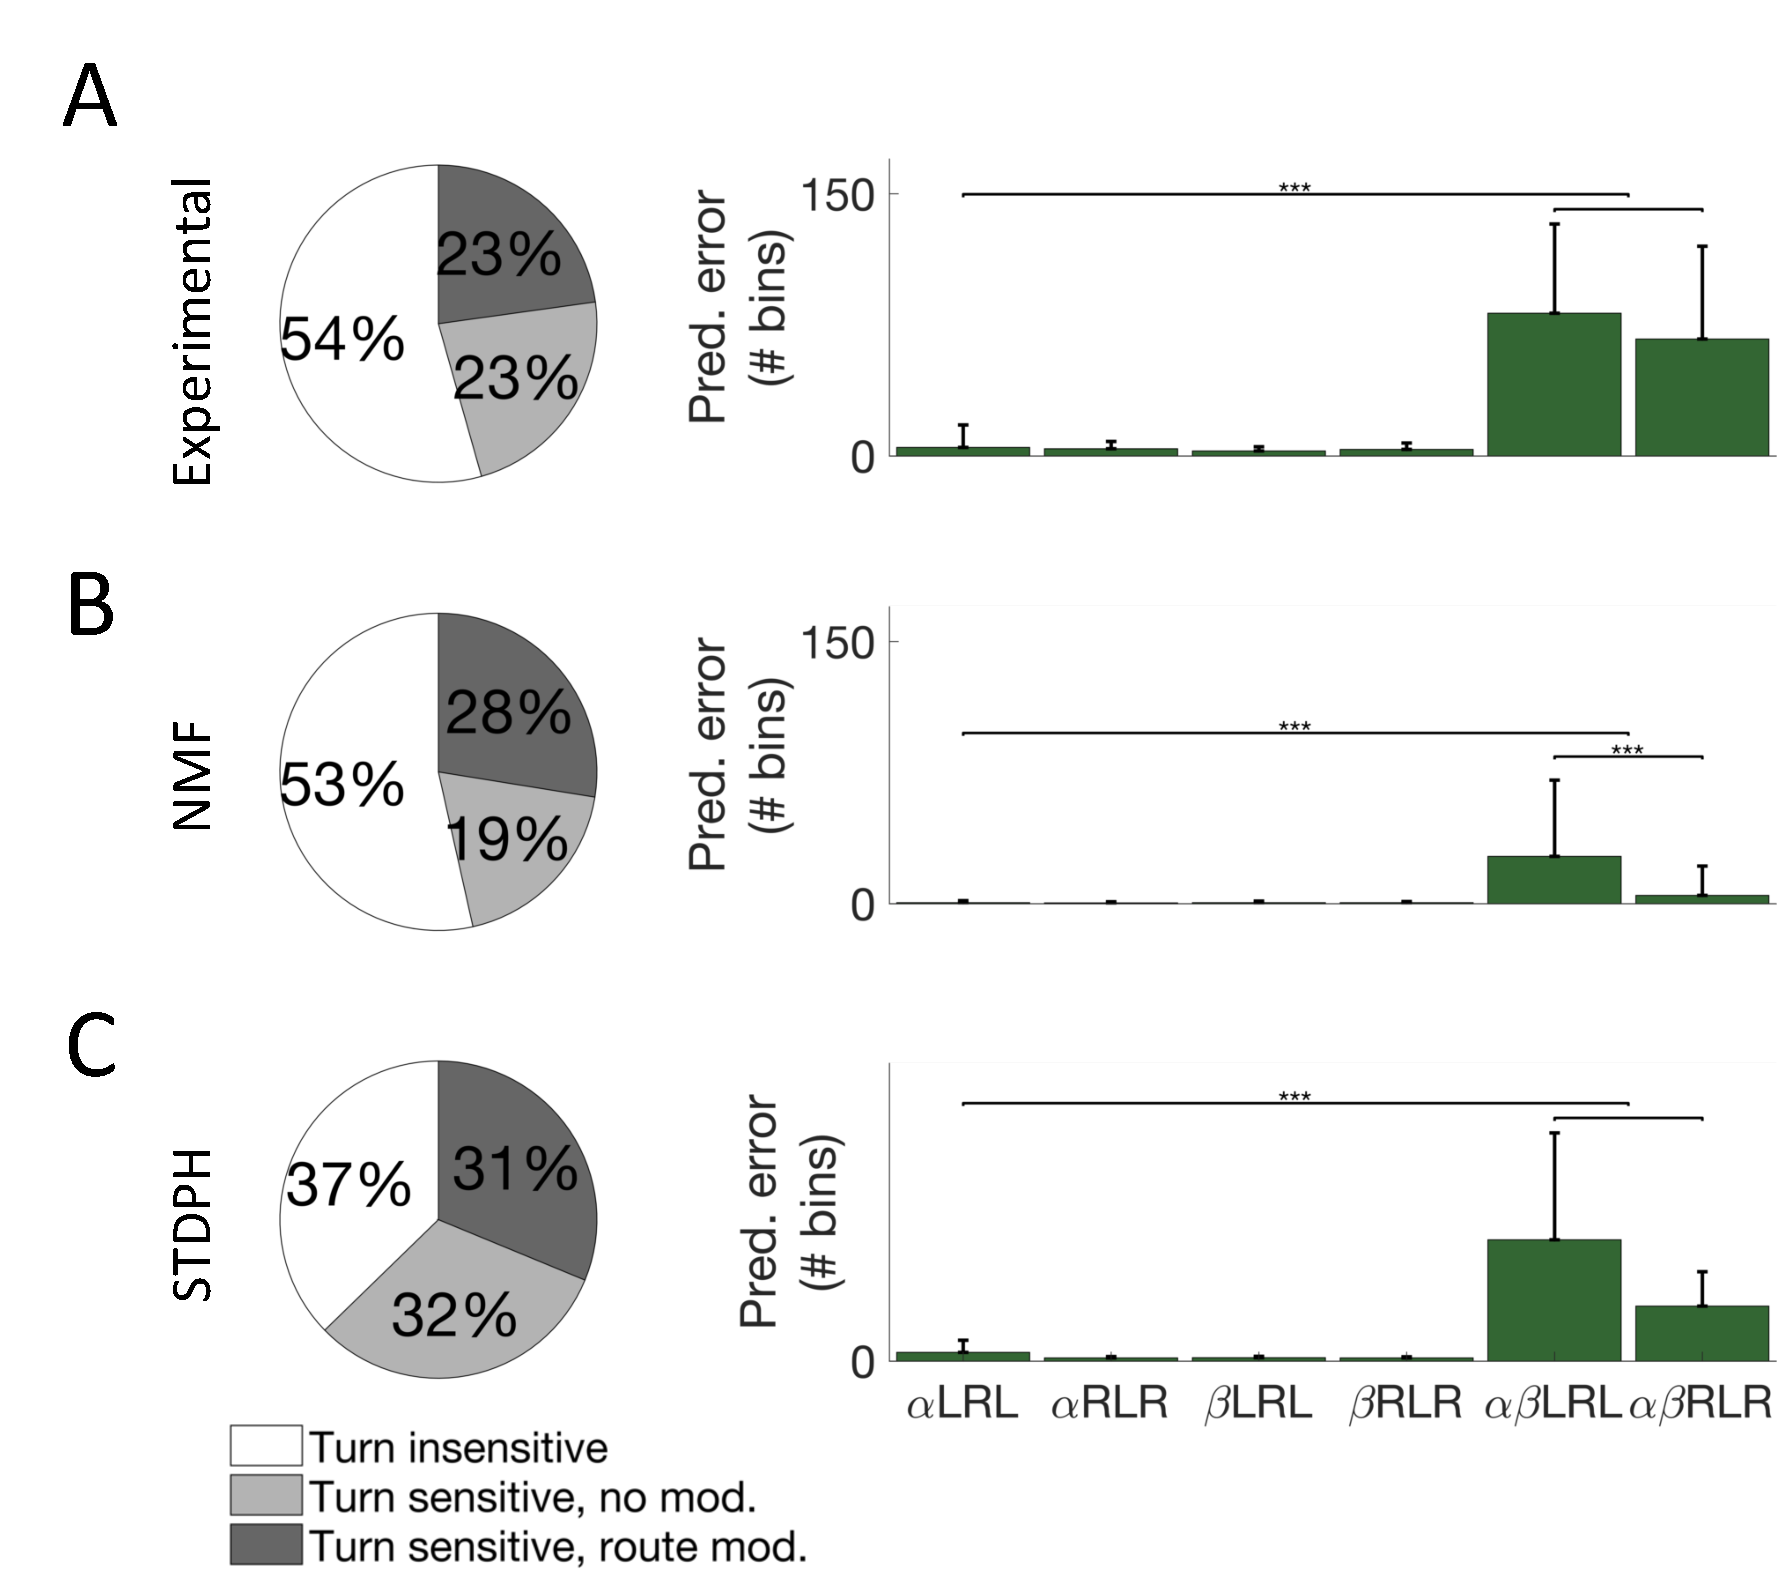
\includegraphics[width=\textwidth]{fig3}
    \caption{Functional neuron type distributions found in the dataset and produced by each model (left columns) and average error corresponding to positional ensemble reconstruction matrices (right columns). Separate allocentric positions of the track are represented by the symbols $\alpha$ and $\beta$. Reconstructions between the track positions are represented by $\alpha$$\beta$. There were two possible routes associated with each track: an outbound run consisting of a left-right-left (LRL) turn sequence and an inbound run consisting of a right-left-right (RLR) turn sequence. A) Experimental data from \cite{AlexanderNitz2015}. B) Simulated using NMF. C) Simulated by evolving STDPH parameters to fit experimental data from \cite{Rounds2016}.}
	\label{fig:NMF|RSC}
\end{figure} 



These findings lend credence to our proposal that \ac{NMF} and \ac{STDPH} 
are functionally equivalent.
Furthermore, the matrix \textbf{W} produced by \ac{NMF} when applied to the \ac{RSC} dataset was qualitatively similar to the synaptic weight matrices produced by 
simulations in which \ac{STDPH} was evolved to match the same dataset.

% This evidence suggests that there is merit to comparing
% synaptic weights generated with both \ac{NMF} and \ac{STDPH} to
% synaptic connections in the brain.
% In cases where synaptic weights from biological neurons are unavailable,
% simulated weight matrices could be used to advance theories of brain areas 
% with complicated neuronal responses
% (such as \ac{MSTd} or \ac{RSC});
% for example, by predicting neuronal responses to novel stimuli
% and simulating experimental perturbations.


% \ac{NSC} may have emerged as a general encoding strategy is because it can be approximated by certain forms of synaptic plasticity, such as \ac{STDPH}, under certain conditions. STDP, or spike-timing dependent plasticity,\emilyNote{this sentence implies STDPH -> NSC, but relationship could be other way: NSC->STDPH, so be careful with this idea here...}
% %is a learning mechanism by which synaptic weights are potentiated or depressed based on the precise spike times of pre- and post-synapic neurons. \ac{STDP} 
% is a learning mechanism that has been found in many brain regions and is generally assumed to take place in some form in every brain region. \emilyNote{much citations, very need} However, there may be many kinds of implementations of STDP in the brain that could also impose other statistical constraints in addition to nonnegativity. In a modified \ac{STDPH} learning rule, STDP is complemented by a homeostatic synaptic scaling mechanism that may give rise to a biologically realistic implementation of \ac{NMF}. In this view, a specific synaptic weight
% (i.e., an element in \textbf{W})
% is modulated depending on the activity of a presynaptic neuron over time
% (i.e., a row in \textbf{V})
% and the activity of a postsynaptic neuron over time
% (i.e., a column in $\mathbf{H}^T$).
% Here, the dimension that used to encompass a number of observations or stimuli $S$
% is now interpreted as time $t$.
% In this context, a row of \textbf{V} corresponds to a specific neuron's firing
% rate over time.
% Then the synaptic weight update rule of \ac{STDPH}
% is mathematically equivalent to an iteration step in \ac{NMF}
% (see \citep{Carlson2013} for a mathematical proof).
% This bestows upon a pre-postsynaptic neuron pair the ability to implement
% \ac{NMF} literally through learning.\emilyNote{more citations; maybe kris would have some} This process is exemplified in Figure \ref{fig:NMF|STDPH}. However, there are multiple kinds of homeostasis that may exist in the brain as well, which may change the nature of the statistical constraints on the pre- and post-synaptic neuron pairs. 

% Another reason might be the fact that \ac{NMF} can be approximated
% by \ac{STDPH} \citep{Carlson2013} (Box 2).

% \mikeNote{words whole para}
% \Ac{STDP} is a synaptic learning that modulates synaptic weights based on the
% precise firing of pre and postsynaptic neurons.
% \Ac{STDP} is ubiquitous in the brain (even in the adult brain, right),
% but it comes in many different forms.
% In one particular form, where \ac{STDP} is complemented with
% homeostatic synaptic scaling (which we refer to as \ac{STDPH}),
% it might be equivalent to \ac{NMF}.




% Do we ever actually define sparsity?


% % I'm pretty sure readers of a high-impact journal such as Trends in Neurosciences
% % have heard of lateral inhibition before...
% In addition to nonnegativity constraints,  sparsity in the neural code may be enforced by lateral inhibitory connections in which excited neurons  inhibit their neighbors such that only a few neurons remain sufficiently active in response to a stimulus, resulting in enhanced  sensory perception. This kind of anti-Hebbian learning can be implemented using the Oja learning rule, which can then be used to control the sparsity of the neural code to ensure a robust and fault-tolerant, but also energy efficient, encoding. % Also Oja approximates PCA and that may or may not be relevant. 
% This conception of STDPH as a biological implementation of NMF implies that the weight matrices generated by an NMF decomposition should be equivalent to those learned by biological neurons in the brain, and by artificial neurons in SNNs under STDPH. Comparing the weight matrix \textbf{W} from \ac{NMF} once again
% to empirical data makes it clear that there is a strong correspondence, and in the case of \ac{V1}, synaptic weights recovered with \ac{NMF} closely resemble biological weight matrices in cat \ac{V1}. Moreover, similar results can be achieved with \ac{STDPH}. 
% %iffy on this
% The structures of synaptic weight matrices in higher cortical regions are unknown;
% \mikeNote{Sure, we can make this prediction. But it is not testable}
% however, we predict that comparisons of the matrix W generated by NMF and STDPH for the simulated RSC data would resemble the actual weight matrix associated with RSC neurons in the biological brain.



% \subsection{Retina}
% \label{sec:evidence|vision|retina}

% % Using \ac{NMF} to explain single-trial spike trains in the retina \citep{Onken2016}.

% % Overview:
% % - A variety of methods were applied to retinal ganglion cells  in order to analyze their firing patterns
% % - These methods included spatiotemporal PCA, ICA, and NMF, but also included Tucker-2 factorization with orthogonality or non-negativity constraints (yielding orthogonal Tucker-2 and space-by-time NMF).
% % - Space-by-time methods were more accurately able to decompose firing patterns into modules or basis vectors
% % - While orthogonal Tucker-2 was able to pick up on variance between patterns that allowed for better reconstruction (more efficient and more robust), space-by-time NMF picked up on stereotyped patterns and resulted in more consistent and generalizable modules
% % - (What does this actually mean...?)

% %  Means that for patterns of stimuli with spatial and temporal components, space-by-time techniques will be better at representing the underlying structure of the data. But if patterns are inseparable in space/time, then you don't need tensor factorization.
% % ...So what happens in the brain? Presumably both kinds of stimuli are possible. Does the brain have both spatiotemporal coding and tensor factorization style coding? What circumstances dictate when which is employed, if so?

% In seeking a scalable way to analyze population codes for large numbers of neurons in both the spatial and temporal dimensions, researchers applied spatiotemporal PCA, ICA, and NMF to both simulated spike trains and neurophysiological spike trains recorded from the retinas of salamanders. %Poor axolotls. :( 
% They also applied tensor factorization methods with either orthogonality or non-negativity constraints. Tensor factorization is a method that decomposes data into separated spatial and temporal domains such that you get separate basis functions (or "modules") for each. This is important because neurons may vary their responses in the spatial domain based on location (neurons closer to one another may share common inputs, for example), and in the temporal domain by varying their response patterns over time.  By decomposing firing rate patterns into spatial and temporal domains separately, a neuron's spatial and temporal contributions to the population code can be elucidated \citep{Onken2016}.

% The different techniques were applied to simplified simulated datasets in order to test how well each technique could extract the 'ground truth' of a known pattern, either separable or inseparable in space and time. First the researchers applied techniques to simulated datasets with a high signal to noise ratio (SNR) that were separable in space and time, which should be easily distinguishable. Blocks of time in which neurons fired at 300 Hz were randomly interspersed amongst background firing of only 2 Hz.  In this case, only spatiotemporal NMF and space by time NMF (Tucker-2 tensor factorization with non-negativity constraints) could recover the underlying ground truth in the pattern.  Given a low SNR (30 Hz with background firing of 2 Hz) pattern that was separable in space and time, only space-by-time NMF was able to faithfully recover the underlying structure. When a pattern was inseparable in space and time (SNR was again 300 Hz to 2 Hz), space by time NMF could no longer recover the underlying blocks, but spatiotemporal NMF could, suggesting that NMF is a better technique for decomposing firing rate data into its fundamental components than PCA or ICA.

% The researchers also looked at the differences between the Tucker-2 factorization methods with non-negativity or orthogonality constraints in their ability to recover stereotyped and repeated firing patterns in the data. They found that orthogonal Tucker-2 factorization led to more robust and efficient representations, but they were overall less compact, and they did not lead to stable modules that recovered stereotyped firing patterns - instead, this kind of factorization yielded modules that were less consistent and seemed to extract differences in activation pattern across stimuli (as opposed to commonalities). The authors note that all other methods with statistical constraints had the same inconsistency, suggesting that non-negativity is the most promising constraint for extracting stereotyped firing.

% Following testing on known ground truth, the researchers recorded spikes from in vitro retinal ganglion cells  while the cells were exposed to natural images (either still photographs or videos). They then applied the Tucker-2 factorization methods (with orthogonality or non-negativity constraints) to the recorded datasets. The results were similar to the simulated data case; space-by-time NMF could decompose the data into compact and sparse representations with three temporal modules and eight spatial modules, while orthogonal Tucker-2 yielded four temporal modulates and sixteen spatial modules. While orthogonal Tucker-2 was also more accurate than space-by-time NMF for correctly decoding the activity, the resulting modules were again inconsistent and relied more on differences between patterns of firing rather than extracting similarities in firing pattern. The modules resulting from space-by-time NMF, on the other hand, were more consistent and more representative of an underlying stereotyped pattern of firing in addition to being a sparser and more compact representation. 
% % Is it important to talk about the contribution of first spike latency and redundancy in spatial/temporal coding?

%  The researchers used the time-only and space-only information to decode the natural images presented to the RGCs and found that decoding was far less accurate when information from the spatial dimension was missing, but only slightly less accurate (though still statistically significantly so) when information from the temporal domain was missing. Further experiments using first spike latency (in which space-by-time NMF was applied to an altered dataset where all spikes except the first one for each neuron and trial were deleted) suggested that information is carried redundantly by spike timing and rate coding, because decoding error was on par with space-by-time NMF under these conditions. Further investigations in which RGCs were shown flashed gratings in different orientations revealed that spike timing is especially important for discriminating fine differences in images that fall within the boundaries of a receptive field.
 
%  The authors conclude that NMF is a biologically plausible tool for spike train analysis (the outputs of NMF can be directly interpreted as synaptic weights, and they are highly generalizable), and that the reason it has been used in a limited number of cases may be due to the fact that spatiotemporal NMF does not perform robustly under certain conditions; specifically, conditions where there is significant overlap in firing patterns and when there is a low SNR. By using space-by-time NMF, these problems can be overcome, and also allows for the analysis of the spatiotemporal structure of neuronal firing patterns. We suggest that the good performance of space-by-time NMF in terms of its ability to extract a sparse and highly compact representation of the underlying structure of a neural code is further evidence that the brain may be employing similar methods for handling the high dimensionality of incoming stimuli. However, since not all patterns are separable in space and time, it is an open question how the brain might handle incoming information under such conditions.

% "The advantage of the non-negative decomposition was its ability to robustly find compact and directly interpretable firing patterns that occur across many different kinds of stimuli. These patterns can be used as basis functions to linearly build a set of code-words of firing patterns, complementing existing approaches [98, 99]. The shape of these firing patterns can thus be examined to provide important information about the structure of the neural code, for example to make hypotheses about the spatial and temporal resolution at which a neural code should be read out. As an example of the information that these modules may give, the structure of spatial modules extracted from RGCs suggests that informative patterns of simultaneous firing come from localized groups of neurons whose receptive fields are close together and that have similar stimulus tuning. "




% \subsection{Early visual cortex}
% \label{sec:evidence|vision|V1}
% % MB TODO

% A popular theory about early visual cortex function is that of sparse coding.

% Sparsity has been proposed as a general principle for the visual cortex. Barlow has argued for sparsity
% on the grounds that only a small proportion of neurons in V1 (and elsewhere??) fire in response to a
% given image and hence the response is ”sparse”. This is desirable for neurons because it means that only
% a few of them need to be active and expend energy (the brain consumes more energy than the rest of the
% body).

% The principle behind sparse coding is that the vision system has an over-complete set of basis functions.
% It tries to represent each image in terms of a small set of these functions. This over-completeness means
% that the the basis functions can be tuned to interesting features of the image. As mentioned above, the
% sparsity principle can also be used to learn receptive fields from natural images (refs!!).

% This sparsity criteria was developed by Olshausen and Field as a way to learn receptive fields of
% neurons \citep{OlshausenField1996}. It gives a reconstruction criteria that can be extended to multiple images and used to learn receptive fields.

% This results in receptive field models which are similar to those measured \citep{OlshausenField1996}. Note that similar
% receptive fields can be obtained by assuming a similar model for the image, see equation (7), but imposing
% different assumptions on the form of the si
% . In particular, independent component analysis (ICA) gives
% similar receptive field models \citep{vanHateren1998}.
% \cite{Hyvarinen2010} explained this by showing that both types of models –
% L1 sparsity and \ac{ICA} – both encourage that the $s_i$ are strongly peaked at 0, 
% but can occasionally have
% large non-zero values (this contrasts with the Gaussian model – e.g. pseudo-inverse – where the 
% $s_i$ are strongly discouraged from taking large values).



% % Topographic NMF: \url{http://www.mitpressjournals.org/doi/pdf/10.1162/neco.2009.03-08-722}
% % It seems like they're adding space to the NMF computation, which might make this kind of similar to the space-by-time NMF algorithm discussed in the retina paper? Am I thinking about that correctly? -Emily






% \subsection{Audition}
% \url{https://www.ncbi.nlm.nih.gov/pmc/articles/PMC4747712/}
% Wondering if NMF could explain the feature composition

% \subsection{Speech}
% S. Zayd Enam, Michael R. DeWeese: Spectro-Temporal Models of Inferior Colliculus Neuron Receptive Fields 
% Sparse codes for speech spectrograms qualitatively match properties of receptive fields of Inferior Colliculus (ICC) neurons. We find sparse codes of speech-spectrograms are well described by one of four models and we find that these models also fit ICC spectro-temporal receptive fields (STRF) well. Further, our models are able to express time-frequency inseparable receptive fields (e.g. frequency sweeps) that previous models were unable to satisfactorily describe. Our models allow the accurate characterization of high-dimensional STRFs with more natural parameterizations of the neuron's behavior. \emilyNote{Not sure we'd want to cite this paper? "To determine STRF model classes we first fit model classes to the sparse codes of speech-spectrograms using non-linear least squares methods"}


% \subsection{Olfaction}

% % Structure this as...
% % 1) There are lots of possible odor combinations and sparse ensemble of neurons to encode them
% % 2) The sparsity of the olfactory code is poor in information and metabolically costly, so functional significance is unclear
% % 3)  Granule cells may complement the code of the mitral cells because they are sparse/incomplete representations
% % 4) This might result in 'explaining away' approach by this system as described in the SNN paper, which was able to detect combinations of odorants very accurately
% % 5) Brief description of causal inference in spiking via explaining away and how it relates to NMF?


% Check this Drugowitsch paper:
% Causal Inference and Explaining Away in a Spiking Network
% Rubén Moreno-Bote \& Jan Drugowitsch, Scientific Reports
% \url{https://www.nature.com/articles/srep17531}

% Also Koulakov and Rinberg:
% Sparse incomplete representations: A novel role for olfactory granule cells
% \url{https://pdfs.semanticscholar.org/ed52/1b318aa68fe8ec71fb9a84d5e577130c6893.pdf}

% It's \emph{almost} doing \ac{NMF},
% and suggests that such a computation might underlie odor classification.

% Antennae -> antennal lobe -> mushroom body (Kenyan cell)
% only 34 output neurons for odor classification
% any given odor activates a unique and sparse ensemble of kenyan cells

% From Graziano \& Aflalo: In this review, the authors suggest that at least some sectors of the cortex do not have a simple global ordering and are better understood as a result of a reduction of a highdimensional space onto the cortical sheet. The cortical motor system may be an example of this phenomenon. The authors discuss a model of the lateral motor cortex in which a reduction of many parameters onto a simulated cortical sheet results in a complex topographic pattern that matches the actual monkey motor cortex in surprising detail. \citep{GrazianoAflalo2007} Source:

% \url{https://www.princeton.edu/~graziano/neuroscientist_07.pdf}
% \url{http://ieeexplore.ieee.org/document/7229368}


% % \subsection{Somatosensory cortex}
% % % MB probably cut...

% % Chapin \& Nicolelis (1999). Journal of Neuroscience Methods. Principal component analysis of neuronal ensemble activity reveals multidimensional somatosensory representations.
% % Recorded neurons from rat somatosensory cortex and applied PCA to the data. Found multidimensional somatosensory receptive fields.
% % From abstract: "The fact that this transformation is mathematically equivalent to the general Hebb algorithm in linear neural networks provided a major rationale for performing it here on data from real neuronal ensembles."


% % THIS SECTION HAS BEEN EXCLUDED FROM THE PAPER



% \label{sec:discussion}
% \subsection{NSC as a ubiquitous coding strategy}
% \ac{NSC} may have emerged as a ubiquitous strategy because reasons
% \subsection{Neurons are nonlinear. Why nonlinear dimensionality reduction?}
% Some researchers say nonlinear reduction techniques do not give you a rich enough representation but we disagree because we did some stuff and it worked and also more reasons.
% \subsection{Where do we go from here?}
% Neuroscience is in a position to actually start looking at RFs in more obscure, hard to reach areas of the brain and we are getting better at looking at the structure of synapses too. Propose new studies.

% % \mikeNote{TODO: better title, maybe use subsection titles instead}


% % % We are currently at 4000 words without the discussion and excluding text boxes/glossary.
% % %...limit is 2500


% % The Discussion section is still a mess.
% % I have compiled some thoughts and notes that I think would be worth incorporating.


% % Let's make sure we touch on the world view (and publications) of the big players in the field: Jonathan Pillow, Surya Ganguli, Maneesh Sahani, Liam Paninski, Mitya Chklovskii(?), Terry Sejnowski(?), Jonathan Victor(?), Wolfgang Maass(?)
% % %  Wolfgang Maass paper on probabilistic inference:
% % % http://eneuro.org/content/eneuro/early/2016/03/25/ENEURO.0048-15.2016.full.pdf
% % % Idea: WTA circuits can pull out underlying statistical structure of training data and can generalize from it
% % %  Seems like Maass might agree with us: "From the perspective of some theories of neural coding and computations it would be desirable that different neurons in a local network can encode independently of each other specific features of a sensory stimulus. However virtually all simultaneous recordings from many neurons within a local patch of cortex suggest that the joint activity patterns of nearby neurons are restricted to variations of a rather small repertoire of spatio-temporal firing patterns."
% % % From  "Searching for principles of brain computation " in current opinion in behavioral sciences


% % % For Pillow, maybe this paper is a good one to talk about...
% % % Has to do with extracting statistics from spike trains, but they argue most dim. red. methods don't capture enough info
% % % https://arxiv.org/pdf/1610.08465.pdf


% % % For Ganguli, we have the compressed sensing paper...

% % %  Seems like Sahanhi emphasizes nonlinearity...
% % % http://www.gatsby.ucl.ac.uk/~maneesh/papers/luecke-sahani-2008-jmlr.pdf


% % %...and if anyone has papers from any of these authors listed that they feel must be mentioned, please list them here.


% % \emilyNote{Kris: mapping synapses that generate activity. Right on the cusp of being able to compare weight matrices deep in the brain, we could propose a study.}




% % In more detail:
% % % From the Ganguli paper
% % The problem of storing, communicating, and processing high-dimensional neural activity
% % patterns, or external stimuli, presents a fundamental challenge to any neural system.
% % This challenge is complicated by the widespread existence of convergent pathways,
% % or bottlenecks, in which information stored in a large number of neurons is often
% % compressed into a small number of axons, or neurons in a downstream system.
% % For example, $1$ million optic nerve fibers carry information about the activity of
% % $100$ times as many photoreceptors.
% % Only $1$ million pyramidal tract fibers carry information from motor cortex to the
% % spinal cord.
% % And corticobasal ganglia pathways undergo a $10$ to $1,000$ fold convergence.

% % Another bottleneck is posed by the task of working memory, where streams of sensory
% % inputs must presumably be stored within the dynamic reverberations of neuronal circuits.
% % This is a bottleneck from time into space: Long temporal streams of input must be stored
% % in the instantaneous spatial activity patterns of a limited number of neurons.



% % \subsection{How could a population of neurons implement dimensionality reduction?}

% % % Interesting note in the Bar-Gad paper: How do neurotransmitters help in shaping the statistical constraints on neural computation?
% % When both input neurons, conveying the feature and its opposite, are connected to the same output neuron using the same neurotransmitter (and therefore the same constraint).  



% % % same here
% % Regularization techniques used by statisticians to learn
% % high-dimensional statistical models from limited amounts of data
% % can also be employed by synaptic learning rules to efficiently search
% % the high-dimensional space of synaptic patterns
% % in order to learn appropriate rules from limited experience.

% % Indeed, it has long been known that neural networks can perform
% % efficient dimensionality reduction using competitive Hebbian learning rules
% % for inter-layer connectivity \citep{Oja1982} and anti-Hebbian rules
% % for the lateral inhibitory intra-layer connectivity
% % \citep{DiamantarasKung1996}.
% % Such a setup leads the network to extract in the weight vector a direction
% % aligned with the first principal component of the input space
% % (in the sense of \ac{PCA}).



% % Also cool to think about 
% % that solving \ac{NMF} is considered to
% % be NP-hard. If \ac{STDPH} can do it, this might be a biological
% % way to solve an NP-hard problem!





% % \subsection{The neuronal code is non-linear. What's with all the talk about \emph{linear} dimensionality reduction?}

% % \mikeNote{Not sure if we need this section - thoughts?}
% % \emilyNote{I think we can sum all this up in a paragraph that might make it into the discussion, but I think a whole section for it is too much.}
% % \mikeNote{Definitely. It was more of an attempt to explain my current line of thinking to the group. :)}
% % Here's one way to think about things:

% % Think of a neuron as this complex, high-dimensional, non-linear machine of which we don't know
% % the input-output function. In fact, it's not feasible to know its input-output function.
% % It's not possible to enumerate all stimuli that would trigger a neuron to respond - this space
% % is simply too large to map out.
% % If you wanted to have a mathematical function that describes a neuron's response to an arbitrary
% % input stimulus, it would have an enormous number of input variables,
% % and the response would be highly non-linear. So this is not feasible.

% % Instead, what we do is we simplify.
% % 1) We might limit our analysis to a small number of input variables, and see how the neuron
% % responds to those.
% % 2) We might use linear techniques to estimate a neuron's response.
% % 3) A combination of 1) and 2).

% % In all cases, we end up with a simplified version of a neuron's response function -
% % or, if you want: a first-order approximation of a neuron's \emph{true} response function.
% % In fact, the traditional ``receptive fields'' of visual neurons are actually retrieved with
% % linear techniques, such as the spike-triggered average:
% % These techniques can only recover the linear relationships of the neuronal response to input
% % data.

% % So when we compare \ac{NMF} representations to classical receptive fields, we are essentially
% % comparing it to these linear receptive field estimations.
% % If we get a good match, it would be foolish to say that a neuron actually implements \ac{NMF},
% % and that \ac{NMF} is all there is to it.
% % If a neuron is a Taylor series, \ac{NMF} is simply a good representation of its first-order term.

% % Don't know if this is useful/relevant:
% % \url{https://papers.nips.cc/paper/5263-low-dimensional-models-of-neural-population-activity-in-sensory-cortical-circuits.pdf}
% % \url{https://pdfs.semanticscholar.org/3ed7/dd40d10cddc1a0715cc0f3493f0be290e34a.pdf}





% % \subsection{How does dimensionality reduction fit with divergent pathways?}

% % % From Ganguli
% % Like convergence, the expansion of neural representations through divergent
% % pathways is a widespread anatomical motif.
% % For example, information in $1$ million optic nerve fibers is expanded into more than
% % $100$ million primary visual cortex neurons.
% % Also, a small number of mossy fibers in the cerebellum target a large number of
% % granule cells, creating a $100$-fold expansion.

% % From Micah's paper: This is
% % interpreted (see e.g. [Olshausen and Field 1996, 1997]) as V1 neurons forming a sparse
% % overcomplete representation of the visual input, with receptive fields of nearby neurons being
% % non-orthogonal and with only a relatively small fraction of neurons being active at any given
% % instant for natural stimuli.
% % \url{http://www.annualreviews.org/doi/pdf/10.1146/annurev-neuro-062111-150410 }

% % Motivated by the observation that in the hippocampus, lots and lots of inputs are coming in through the entorhinal cortex (EC) to the dentate gyrus (DG) where inputs are orthogonalized and made very sparse. 

% % After the DG, inputs are passed into the CA1-CA3 regions of the hippocampus, areas which contain place cells, are thought to hold a representation of an allocentric cognitive map, and also is thought to act as an autoassociative network.

% % The CA1-CA3 regions use the sparse representations from the DG to generate autocompleting representations.

% % Long story short:
% % If you sparsify the representation, you might end up with a representation that requires more
% % neurons than you had to begin with.
% % If you look at the number of neurons, you might prematurely
% % conjecture that the dimensionality went up.
% % But if you look at the embedding, 
% % it might effectively be simpler (lower-dim) 
% % than the input.






% % \subsection{How do we fit with popular theories of brain function?}

% % Data compression shows up in a lot of theories of brain function, but in various forms
% % (e.g., information maximization in efficient coding; free-energy minimization in Friston's stuff;
% % maybe look up Grossberg, Poggio; Heeger put out a new theory, but doesn't touch on compression).
% % More complete theories of brain function usually have other parts, such as prediction and feedback.


% % Would be good to discuss how we relate to Alan Yuille compositional learning stuff.
% % Also: compressed sensing, efficient coding, free energy.

% % Also, \ac{NMF} is related to k-means clustering (check Wikipedia),
% % multinomial PCA (check Wikipedia),
% % and spectral clustering \citep{PehlevanChklovskii2014,Ding2005}.

% % Also, it fits the idea that compression is among the fundamental principles of
% % cortical computation \citep{Richert2016} - could be a nice way
% % of ending the paper: information compression is fundamental!




\section{Concluding remarks and future directions}
\label{sec:conclusion}

In this article,
we have argued that a variety of neuronal response properties can
be understood not as an emergent property of efficient population coding
based on dimensionality reduction and sparse coding.
We offer three testable predictions of this theory:

First, we predict that parts-based representations can explain
\acp{RF} of neurons in a variety of brain regions,
including but not limited to those brain areas discussed here (i.e., V1, MSTd and RSC). In agreement with the literature on basis function representations
\citep{PougetSejnowski1997,PougetSnyder2000,Poggio1990},
we expect parts-based representations
to be prevalent in regions where neurons
exhibit a range of tuning behaviors \citep{Beyeler2016},
display mixed selectivity \citep{Fusi2016,Eichenbaum2017},
or encode information in multiple reference frames \citep{AlexanderNitz2015,Rounds2016}.

Second, where such representations occur, we expect the resulting
neuronal population code to be sparse,
in order to encode information both accurately and efficiently.
Sparse codes are ideally suited for such an encoding, as they offer
a trade-off between 
dense codes (where every neuron is involved in every context,
leading to great memory capacity but suffering from cross talk among neurons)
and local codes (where there is no interference, 
but also no capacity for generalization) \citep{Spanne2015417}.

We also speculate that there may be an important relationship between sparse and distributed coding. Barnes et al. \citep{barnes1990chapter} observed that output from the hippocampus was expressed as a much more distributed code, while the coding scheme within the hippocampus proper was sparse. They suggested that sparse coding might be employed to increase the storage capacity of the region, consistent with our proposed framework. Sparse and distributed codes may represent two sides of the same coin, evidenced by anatomical bottlenecks, in which the brain utilizes synaptic expansion when transmitting information between brain regions and synaptic reduction and sparsification for information storage within regions. \emilyNote{moved reduction/expansion thing here, may or may not fit.}
\mikeNote{Why not, don't know where else it'd fit. Maybe we should a ref for compressed sensing.}

Third, we propose that \ac{STDPH} is carrying out a similar function to \ac{NMF},
and may be attempting to approximate the linear \ac{RF} properties of
neurons participating in sparse, parts-based representations
throughout the brain. STDPH and NMF can effectively produce NSC.
With the emergence of computational tools developed
to understand the neural code 
in high stimulus dimensions \citep{PillowSimoncelli2006},
we expect to see qualitative similarities between empirically observed
\acp{RF} and those recovered by \ac{NMF} and \ac{STDPH}.
Such findings would be consistent with the idea that neurons
can perform statistical inference on their inputs via
Hebbian-like learning mechanisms
\citep{Nessler2009,Carlson2013,MorenoBoteDrugowitsch2015,Oja1982}.



In summary, we suggest that the evidence reviewed in this paper may indicate that dimensionality reduction through nonnegative sparse coding, implemented by synaptic plasticity rules, may be a canonical computation throughout the brain. Initial experiments using STDPH and \ac{NSC} indicate that they may be functionally equivalent, which is backed by computational evidence in which \ac{NSC} and \ac{STDPH} were applied to an experimentally recorded dataset. In summary, \ac{NSC} offers a promising theoretical framework to further our understanding of how high-dimensional data is encapsulated by the often complex and nonlocal nature of cortical computation.



% First, we predict that the receptive fields for neurons that have historically been hard to study due to their location in the brain will prove to yield parts-based representations, consistent with the proposed framework. 
% Second, we predict that in regions where such representations occur, there will be sparse representations of high-dimensional input spaces, especially where there are anatomical bottlenecks.
% Our third prediction stems from the theoretical observation that a highly sparse (local) code, a neuron's response will encompass a highly specific and accurate representation of its inputs, but will not be generalizable to noisy, incomplete, or otherwise altered versions of those stimuli. On the other hand, a dense code (in which all neurons participate in the representation of a set of incoming stimuli), the representation is highly generalizable and accurate, but inefficient because it is not sparse. A sparse code is a compromise between these two extremes and determines the degree to which a representation is efficient and generalizable \cite{Spanne2015417}. Thus we predict that the sparsity of the code in a given brain region will predict the trade-off between the accuracy and efficiency of the code. Finally, we predict that, as our understanding of connectivity in hard-to-reach brain regions improve, there will be qualitative similarities between them and those matrices generated by computational learning methods such as \ac{STDP} and \ac{NMF}, rendering credibility to the idea that neuronal response properties represent the hidden coefficients associated with synaptic `basis functions.'
% Boxes are to use reference like the main text, but the numbering should start after
% the last reference of the main text.
% Ergo, it makes sense in LaTeX to have the boxes after the main text...so we get
% the numbering right

%  Text Boxes
% • Ideal for providing explanations of basic concepts or theories, giving detailed mechanisms, or discussing case studies.
% • Please cite text boxes in the main text as: (Box 1).
% • Boxes should have a single sentence title (no more than 8 words).
% • Text boxes can occasionally contain small figures and tables. Please number figures or tables within a text box with Roman numerals (e.g. Figure I) and cite the element in the box text.
% • 400 words max per box. 
% • References should be listed in the main reference list, numbered to follow on from the end of the main text.
% • No more than four text boxes per article. 

\section{Box 1: Nonnegative sparse coding (NSC)}
\label{box:NSC}

% Need to keep it under 400 words

\Acf{NSC} combines \acf{NMF},
a linear dimensionality reduction technique from statistical learning,
with sparse population coding from neural network theory
\citep{Hoyer2002,EggertKorner2004}.
\ac{NMF} belongs to a class of methods that can be used to decompose
a multivariate data matrix \textbf{V}
into an inner product of two reduced-rand matrices \textbf{W} and \textbf{H}.
\ac{NMF} assumes that the observed data in \textbf{V} are caused by a collection
of latent factors weighted by nonnegative numbers,
representing both the presence and the intensity of the cause.

In the context of \ac{NSC},
\textbf{V} and \textbf{H} correspond to activation values
of two distinct neuronal populations,
which are connected to each other via synaptic weight values
in \textbf{W}
(Fig.~\ref{fig:NMF|reconstruction}).
Consider a number of data samples $s \in [1, S]$, for example,
in the form of observed firing rates of a population of $F$ neurons.
If we arrange the observed values of the $s$-th observation 
into a vector $\vec{v}_s$,
and if we arrange all vectors into the columns of a data matrix \textbf{V},
then linear decompositions describe these data as
$\mathbf{V} \approx \mathbf{WH}$.
Here, \textbf{W} is a matrix that contains as its columns
a total of $B$ \emph{basis vectors} of the decomposition, 
and \textbf{H} contains as its rows the \emph{hidden coefficients}
that give the contribution of each basis vector in the input vectors.
The difference between \textbf{V} and \textbf{WH} is termed
the \emph{reconstruction error}.

The goal of \ac{NSC} is then to find a linear decomposition of \textbf{V}
that minimizes the reconstruction error,
while guaranteeing that both \textbf{W} and \textbf{H} are sparse.
This can be achieved by minimizing the following cost function
\citep{Hoyer2002}:
\begin{equation}
\min_{\mathbf{W}, \mathbf{H}} \frac{1}{2} ||\mathbf{X} -\mathbf{WH}||^2 + \lambda \sum_{ij} f(H_{ij}),
\end{equation}
subject to the constraints
$\forall ij: \mathbf{W}_{ij} \geq 0$, $\mathbf{H}_{ij} \geq 0$, and
$||w^{(i)}|| = 1$, where $w^{(i)}$ denotes the $i$th column of \textbf{W}.
Here, the left-hand term describes the reconstruction error, which can
be minimized with \ac{NMF},
and the right-hand term describes the sparseness of the decomposition.
The trade-off between sparseness and accurate reconstruction
is controlled by the parameter $\lambda$ ($\lambda \geq 0$), whereas
the form of $f$ defines how sparseness is measured
(a typical choice is the L1 norm on \textbf{H}).

% %%%%%%%%%%%%%%%%%%%%%%%%%%%%%%%%%%%%%%%%%%%%%%%%%%%%%%%%%%%%%%%%%%%%%%%%%%% %

\section{Box 2: Equivalence of NMF to STDPH and neural mechanisms of NSC}
\label{Box:NMFvSTDPH}
% ELR: CLEANED UP STDP BOX.
% 398 WORDS TOTAL WHEN PASTED INTO WORD (INCLUDES CITATIONS, SO IS LIKELY SHORTER IN LATEX).

% First paragraph - STDP  on a single synapse
% Second paragraph - STDP on networks?
\Acf{STDP} is a form of Hebbian learning in which synaptic weight changes
\jeffNote{fix ref}
depend on the relative timing between pre- and post-synaptic spikes (??? cite Bi \& Poo; Song \& Abbott). If pre-synaptic spike counts integrated over a critical window precede those of the post-synaptic neuron, then long-term potentiation (LTP) is induced, strengthening the weight. Otherwise, long-term depression (LTD) is induced, suppressing the weight. STDP is ubiquitous throughout the brain across the lifespan and can take on different forms \citep{Caporale2008STDP,Holtmaat2009STDP}. Simulations of \ac{STDP} can result in runaway feedforward excitation such that produces unrealistic firing rates. To obviate this problem in biology, the brain uses homeostatic mechanisms that modulate synaptic inputs and neuronal firing thresholds \citep{Watt2010}.

\jeffNote{see my ??? above regarding the appropriate STDP references.}
% One well-known homeostatic mechanism is synaptic scaling,
% wherein synaptic efficacy is regulated by neuronal activity
% to prevent runaway increases or decreases in synaptic strength.
We focus on synaptic scaling, a particular form of homeostasis which
multiplicatively scales weights up or down
depending on the average firing rate of the postsynaptic neuron, which has
been demonstrated to stabilize \ac{STDP} \citep{Carlson2013,Buonomano2005,VanRossum2000}.
We refer to this combination of \ac{STDP} and homeostatic synaptic scaling
as \ac{STDPH}.

% \mikeNote{I guess this paragraph should be tied to the figure I'm supposed to make}
% \krisNote{I referenced figure 2. It's tricky because I don't have room to describe why H and W are 1D (because we only have one output neuron).}

We have shown that, given a network with fewer output than input neurons and full connectivity from the input layer to the output layer, \ac{STDPH} iteratively acts to preserve the information in the first layer with the output layer neurons. Given an input layer of neurons (represented by matrix \textbf{V}) connected to a single output layer neuron (represented by row vector $\mathbf{h^T}$) we have proven that the \ac{STDPH} rule iteratively updates the synaptic weights in \textbf{w} in such a way as to minimize the reconstruction error of $|\mathbf{V} - \mathbf{wh^T}|$, and that the \ac{NMF} update rule is mathematically equivalent to the \ac{STDPH} update rule \citep{Carlson2013}.

% \mikeNote{Is $\mathbf{wh^T}$ an outer product or should it be a vector \textbf{v}?}
% \krisNote{NMF Matrix question: $\mathbf{wh^T}$ is an outer product. Explanation:
% Let n = number of input 
% neurons, m = number of time steps, and r = number of output neurons. Let r = 1. Then, 
% $V$ is of dimensionality nxm, $w$ is of dimensionality nx1 (column vector), and $h^T$
% is of dimensionality 1xm (row vector). The problem is I was not consistent with what I
% told you for conventions. I have used bold capital for matrix, bold lower case for column,
% and bold columm transpose for row.}
% \mikeNote{Don't tell me, lol, tell the reader!}


% \mikeNote{I said this in the main text}
% The equivalence of \ac{STDPH} to \ac{NMF} should not come as a particular surprise and in fact
% their similarities were alluded to \citep{Masquelier2010} before the mathematical proof for the
% single neuron case \citep{Carlson2013}.
% The equivalence of \ac{STDPH} to \ac{NMF} can be viewed as analogous to the equivalence of Oja\textsc{\char13}s rule to \ac{PCA} in the following way.
% Oja\textsc{\char13}s rule was developed to stabilize the rate-based Hebbian learning rule
% by introducing multiplicative normalization
% just as homeostatic synaptic scaling was added to \ac{STDP}
% for stabilization \citep{Oja1982}.

% Emily note to self: I already mention this a couple places so I can either work it in or replace it elsewhere
% \krisNote{Although relevant, I'm not sure we'll have room for these two sentences}
% As mentioned in Box 1, \ac{NSC} combines the dimensionality reduction of \ac{NMF}
% with the concept of sparse population codes from neural network theory
% \citep{Hoyer2002,EggertKorner2004}.
% \ac{NSC} can be viewed as an additional constraint on \ac{NMF},
% requiring sparsity in the neural firing, represented in the $\mathbf{h}$ vector.
% Third paragraph can be WTA/lateral inhibition.

To induce sparsity in networks of neurons, there must be a mechanism that causes each output layer to learn a different component of the total information represented by the input layer \citep{Foldiak1990}, which may be achieved by competition among units. Lateral or feedforward inhibition is often used to induce competition in SNNs, since it offers a biologically plausible mechanism to implement a \ac{WTA} architecture \citep{Coultrip1992}, although other groups have suggested that thresholding can also achieve sparse codes \citep{Rozell2008}. Therefore, \ac{NSC} can be attained in a two-layer network with \ac{STDPH} and a \ac{WTA} architecture via inhibitory connections within or between layers. Interestingly, popular implementations of \ac{NMF} (e.g., MATLAB, Scikit-Learn) include a constraint on the L1 norm of \textbf{H} that automatically lead to sparsity. Alternatively, an explicit sparsity level can be incorporated into models of \ac{NMF}, such as in Hoyer\textsc{\char13}s model \citep{Hoyer2004}.

%%%%%%%%%%%%%%%%%%%%%%%%%%%%%%%%%%%%%%%%%%%%%%%%%%%%
% Methods for EA experiments of RSC. This is too long (~470 words).

\section{Box 3: Evolutionary Algorithm and SNN Evaluation}
\label{box:EA}
Evolutionary algorithms are a class of optimization algorithms loosely based on concepts from evolution. A set of individuals (in this case, spiking neural networks, or SNNs) have a set of parameters to be evolved, which are initialized for the first generation with size $N$. The population undergoes a training and a testing phase followed by evaluation as determined through a user-defined function that measures how well individuals in the population meet the desired criteria. The resulting value is the individual’s level of \textbf{fitness}. A certain number of individuals are then chosen as parents for the next generation, and undergo \textbf{crossover} and/or \textbf{mutation} to produce the new population of individuals. This process continues until a good solution is found.
In the experiments in which SNNs were evolved to match electrophysiological data, the population size was $N = 15$. The training phase used trials from the experimental dataset from retrosplenial cortex (RSC), recorded as rats ran along a W-shaped track. At each position along the track, behavioral metrics (linear velocity, angular velocity, allocentric position, and head direction) were recorded along with neuronal firing rates. The track could occupy different positions in the room (two locations in a single recording session, $\alpha$ and $\beta$) and each track position had an associated outbound (a sequence of left-right-left (LRL) turns) and inbound (right-left-right (RLR)) run. The rats completed each run $\sim$20 times ($\sim$20 trials per recording session, 71 in total) for each track position and route combination ($\alpha$LRL, $\alpha$RLR, $\beta$LRL, and $\beta$RLR). We randomly selected trials from half the trials in the dataset for training (the other half were reserved for the testing phase). The testing phase was the same as the training phase except STDPH was disabled. Following testing, we measured correlations between synthetic and electrophysiological activity patterns and chose synthetic neuronal matches for each experimentally observed firing pattern based on the best correlations between them. Following fitness evaluation, we used \textbf{binary tournament selection} to choose three new parents (each parent produced five children) for the next generation of individuals. Each new parent underwent mutation without crossover to produce a new child.
To compare experimental neuronal responses with synthetic ones, we analyzed functional neuron types using methods described in Alexander and Nitz \citep{AlexanderNitz2015}. Activations averaged over trials for every neuron in the population were cross-correlated to reconstruct agent’s position within a route. To reconstruct position with respect to one route (such as in $\alpha$LRL), trials were divided into two sets, even and odd, to measure consistency of response. To reconstruct position between track positions (such as in $\alpha$$\beta$LRL), activations over trials associated with the $\alpha$ track position were averaged and cross-correated with averaged activations over trials associated with $\beta$. High correlations between same positions (e.g., bin 1 (row) and bin 1 (column)) indicate a good reconstruction of position from ensemble activity patterns. Within-position reconstructions (even vs. odd trials) yielded accurate positional reconstructions (low error), but between-position (i.e., $\alpha$ vs. $\beta$ trials) were associated with high error and did not yield accurate reconstructions of position, which suggests that the population differentiates routes situated in different parts of space.


% This Drugowitsch paper seems highly relevant:
% Causal Inference and Explaining Away in a Spiking Network
% Rubén Moreno-Bote \& Jan Drugowitsch, Scientific Reports
% \url{https://www.nature.com/articles/srep17531}

% The spike-based implementation can be interpreted as a noisy
% version of the rate-based network (can it?)

\section{Trends Box}

% 900 character limit with spaces - currently at 879 chars in word
%----

% The Trends box is a short collection of bullet point statements (3-5) that concisely convey to the reader the recent advances in the area, including emerging concepts and/or distinctions, that constitute a main motivation for the discussion developed in the article. 

% \begin{itemize}
% \item As the box aims to focus on recent developments, conclusions and future directions should instead be discussed in the Concluding Remarks section and/or the Outstanding Questions box.
% \item The text in the Trends box may not exceed 900 characters, including spaces. 
% \item The Trends Box is not called out in the text.
% \item The Trends Box does not count towards the total number of allowed display elements in the manuscript (limit of 4).
% \item When submitting the manuscript files via Editorial Manager, please upload the Trends Box as a separate word file using the designated heading.
% \end{itemize}

\begin{itemize}
\item Sparse coding models were developed to describe sensory coding in the visual cortex, but evidence for nonnegative, sparse coding schemes exists for many brain regions.

\item  Current thought conceptualizes neuron function as highly selective for specific inputs for the purpose of performing specialized behaviors, but neurons may instead generalize by performing dimensionality reduction on their inputs in order to represent as much information about incoming stimuli as possible, and their functional behavior may simply be an emergent phenomenon resulting from this computation.

\item New evidence suggests that certain forms of spike-timing dependent plasticity, in conjunction with lateral inhibition, may approximate a form of dimensionality reduction that we call nonnegative sparse coding (\ac{NSC}), which may be a common computation performed throughout the brain.

% \item Recent computational studies suggest that nonnegative sparse codes
% might be more prevalent in the brain than previously thought. 
% \mikeNote{Wooooords}
% \emilyNote{aren't they already considered prevalent? not sure I like this point. Also it seems a lot like the second point.}

% \item Originally developed to describe sensory coding in visual cortex,
% we found evidence for nonnegative sparse coding all over the brain.

% \item We think that NSC can be implemented with spike-timing dependent
% plasticity and homeostasis.

\end{itemize}





% Recent advances in high-dimensional statistics and methods for analyzing brain data
% make this an ideal time for
% new discoveries and theories about
% the statistical properties of information processing in the brain.


% Similarly, the brain itself is a vastly complex nonlinear, highly-interconnected network and neuroscience requires tractable, generalizable models for these inherently high-dimensional neural systems.
\section{Outstanding Questions Box}


% ELR: 2000 character limit with spaces. 
% Currently at 1885.

\begin{itemize}

\item That \ac{STDPH} can approximate \ac{NMF} under certain conditions has been proven for the single neuron case, but whether or not a  SNN with that form of \ac{STDPH} can converge to approximate \ac{NMF} is an open question. Can the proof be extended to apply to networks of neurons?

\item The application of \ac{NMF} to neuron populations is due to the fact that \ac{NMF} with sparsity constraints produces sparse, additive, parts-based representations of the features of an input space. It is established that many regions of the brain employ a sparse coding scheme, but the nature of representations and neuronal receptive fields are far less understood. Do parts-based representations appear in regions other than visual cortex that are also known for their sparsity, especially in higher cortical and subcortical regions?

\item \ac{NMF} produces nonnegative basis vectors that combine additively to represent an input space, which is consistent with the fact that neurons cannot have negative firing rates. However, \ac{STDP} can come in many forms, including inhibitory and neuromodulatory. Are there multiple kinds of dimensionality reduction implemented across the brain, determined by the statistical constraints placed upon the synapses of the region by the specific form of \ac{STDP} on the synapse?

\item Is it possible for a linear dimensionality reduction technique to generate a sufficiently rich and faithful representation of a high-dimensional input space that is practical and useful to the organism, or do more sophisticated forms of dimensionality reduction take place?

\item Does \ac{NSC} take place in every brain region, or just some? 

\item The connectivity in hard-to-reach brain regions is not well studied. Can weight matrices produced by \ac{STDPH} and \ac{NMF} with sparsity approximate the structure and connectivity of that observed in biological brains?

\end{itemize}
% Ok, so apparently the glossary isn't just a list of all acronyms
% Pick a few central terms that are worth explaining
% Limit to 450 words

\section{Glossary}

\begin{itemize}
% list alphabetically
% term in bold, then explain more than just long version of abbreviation

\item \textbf{Basis functions} A lower-dimensional set of linearly independent elements that can represent a high-dimensional input space given a weighted sum of these elements, where the weight of each element is defined by a separate hidden component.

% \item \textbf{Binary tournament selection} A selection strategy for producing new parents for the next generation in an evolutionary strategy. In tournament selection, $x$ individuals are chosen randomly, and then the individual in the subset with the highest fitness is chosen as a parent. This is repeated until the number of desired parents have been chosen. In binary tournament selection, $x = 2$ individuals are chosen at random from the population.

% \item \textbf{Crossover} In an evolutionary strategy, parents chosen to produce the next generation may undergo crossover. Each parent has a value associated with each parameter being evolved. To produce a child, the values associated with a parameter may be swapped at random (using a predetermined threshold) between the parents so that the child has a mixture of both parents' parameter values.

\item \textbf{Dimensionality reduction} The process of reducing the dimensionality of a space to the lowest possible space that encapsulates the variance of the original data via feature extraction. In the case of neuronal firing rate patterns, this means representing all possible firing rate patterns in the brain region using the smallest possible subset of the neurons.

\item \textbf{Factor analysis} A statistical method used to describe variability among observed, correlated variables in terms of a potentially lower number of unobserved, uncorrelated variables called factors (or latent variables).

% \item \textbf{Fitness} In evolutionary strategies, a single value computed with a user-defined function that represents how well an individual in a population meets the desired function that is being evolved.

% \item \textbf{Mutation} In an evolutionary strategy, parents chosen to produce the next generation may undergo mutation. Each parent has a value associated with each parameter being evolved. Each parameter may be randomly altered (according to a predetermined threshold) by selecting a new value from some distribution of values that lie within the established range to produce a new child individual for the next generation.

\item \textbf{Receptive field} The structure and boundaries of an individual neuron's pattern of response to various kinds of incoming stimuli.

\item \textbf{Spike-timing dependent plasticity} A Hebbian-inspired learning rule in which weight updates are computed based on the precise spike times of pre- and post-synaptic neurons that induce either long term potentiation or long term depression in the synapse, depending on whether the total pre-synaptic spike count preceded the total post-synaptic spike count, integrated over a critical temporal window.

\end{itemize}
% \section{Notes}

\subsection{RF overlap}

Individual neurons in visual cortex respond selectively to only a small subset
of stimulus features.
However, certain subpopulations of neurons, such as in a cortical column, share substantial
receptive field overlap.
\url{http://www.jneurosci.org/content/19/10/4046}
For example, across a cortical column, neurons may share stimulus dependence
as a result of sampling the same location of visual space,
having similar orientation preference,
or receptive fields with shared sub-units.
As a result, a substantial fraction of stimulus information can be redundant
across neurons
D. S. Reich, F. Mechler, and J. D. Victor, “Independent and redundant information in nearby cortical neurons,” Science, vol. 294, pp. 2566–2568, 2001


\subsection{State space}
Similarly, the spatial response property of a cell (e.g., the receptive field)
can also be described in terms of locations in the state space that will produce
a response.
A population of neurons will occupy only a small subspace of the state space
(sparse embedding). Together, however, they must be able to represent every incoming
sensory pattern in the state space.
% Every distinguishable receptive field profile is represented in terms of a unique
% direction in the state space. Thus, an array of cells can be considered as an array
% of vectors each pointing to unique locations in the state space.
% Now, many studies have shown that 

% receptive fields in \ac{V1} \citep{Barbieri2015},
% and visual grouping \citep{Cocci2015}.

% Somewhere mention that neurons and neuroscientists might face the same dilemma:
% How to make sense of high-dimensional data.
% Because there's an almost infinite amount of high-dimensional input data,
% you have to come up with a way to extract relevant information.
% Neurons might do this with STDPH, 






The principle behind sparse coding is that the vision system has an over-complete set of basis functions.
It tries to represent each image in terms of a small set of these functions. This over-completeness means
that the the basis functions can be tuned to interesting features of the image. As mentioned above, the
sparsity principle can also be used to learn receptive fields from natural images (refs!!).

This sparsity criteria was developed by Olshausen and Field as a way to learn receptive fields of
neurons \citep{OlshausenField1996}. It gives a reconstruction criteria that can be extended to multiple images and used to learn receptive fields.

This results in receptive field models which are similar to those measured \citep{OlshausenField1996}. Note that similar
receptive fields can be obtained by assuming a similar model for the image, see equation (7), but imposing
different assumptions on the form of the si
. In particular, independent component analysis (ICA) gives
similar receptive field models \citep{vanHateren1998}.
\cite{Hyvarinen2010} explained this by showing that both types of models –
L1 sparsity and \ac{ICA} – both encourage that the $s_i$ are strongly peaked at 0, 
but can occasionally have
large non-zero values (this contrasts with the Gaussian model – e.g. pseudo-inverse – where the 
$s_i$ are strongly discouraged from taking large values).

The fact that features can ``cancel each other out'' using subtraction is contrary
to the intuitive notion of combining parts to form a whole.
Non-negativity ensures that elementary object features combine additively.

However, there are at least two ways in which the standard sparse coding image model
is unrealistic as a model of \ac{V1} simple-cell behavior.
First, each unit $s_i$ in the model can,
in addition to being effectively silent (close to zero),
be either positively or negatively active.
This means that every feature contributes to representing stimuli of opposing polarity;
for example, a unit that codes for a dark bar on a bright background also codes
for a bright bar on a dark background. This in in contrast to the behavior of simple cells
in \ac{V1}, which can only represent one half of the output distribution of a signed
feature $s_i$, as firing rates cannot go negative.
Second, input data in the standard sparse model is double-sided (signed),
whereas \ac{V1} receives the visual data from the \ac{LGN} in the form of separated
ON- and OFF-channels.

Thus, if we would like to transform sparse coding from a relatively abstract model
of image representation in \ac{V1} to a concrete model of simple-cell recoding of
\ac{LGN} inputs, the model must be changed.
First, the input data should consist of hypothetical activities of ON and OFF channels
in response to natural image patches.
Second, all coefficients should be restricted to be non-negative.

\url{https://arxiv.org/pdf/1509.03942v1.pdf}: Dimensionality reduction in V1: This can be interpreted as a principle of dimensionality reduction constrained to optimally independent representation of orientations, in the following sense. As previously observed, V1 does not have a sufficiently high topological dimension to implement all scales/frequencies and orientations over each point, so it has adopted compromises such as the one described by the coverage strategy. On the other hand, if we measure the independence of receptive profiles in terms of correlations, then the maximal independence with respect to orientations can be obtained equivalently by translations at a given distance. This distance can be estimated to grow with the shape index, as described by Figure 11, and reaches the characteristic length of the orientation preference maps at about the cutoff value for the shape index. At that distance, two receptive profiles can then be considered as collecting a sufficiently independent information that justifies a repetition of a new full set of orientations. Say it from another point of view, orientation preference maps may be a way to map a compact variable on the highly redundant sampling space of positions


It is well known since the fundamental studies of Hubel and Wiesel [23, 22] that primary
visual cortex (V1) is one of the first physiological layers along the visual pathway to
carry out geometrical measurements on the visual stimulus, decomposing it in a series of
local feature components. The development of suitable electrophysiological techniques
[43] has made possible to reconstruct the linear filtering behavior of V1 simple and
complex cells, i.e. their spatio-temporal receptive profiles (RPs).
The RPs of orientation-selective cells in V1 have classically been modeled with twodimensional
Gabor functions [24], which basically compute a local approximation of
the directional derivative of the visual stimulus, minimizing the uncertainty between
localization in position and spatial frequency [13]. On the other hand, spatio-temporal
RPs of V1 simple cells can be modeled by 3-dimensional Gabor functions of the form
[11]




In this letter, we propose that sparse, parts-based dimensionality reduction might be a common mechanism to achieve representation of information in the brain. We first explain possible algorithms in the Methods, then list evidence of where this has been found in the brain, and close with our thoughts of how such an algorithm might be implemented in the brain.


If we end up having to define what we mean by dimensionality (what space are we talking about?), this paper’s introduction mentions a bunch of references that talk about how people have defined the dimensionality of a neural system in past works: \url{http://journal.frontiersin.org/article/10.3389/fnsys.2016.00011/full}


This paper (http://jn.physiology.org/content/jn/107/10/2594.full.pdf) discusses spectrotemporal response fields and how many filters are required to describe the stimulus preferences of a neuron in the auditory cortex. Apparently, the visual and auditory cortices are pretty different in this regard. Would be useful to  know more about this in other brain regions.



However, ``dimensionality'' in the literature has been interpreted in a variety of ways.
For example, \cite{DurbinMitchison1990} suggested that cortical maps can be understood
as a dimension-reducing mapping from high-dimensional parameter spaces
onto the surface of the cortex,
such that local computations in parameter space can be performed locally in cortex.
Others have applied the term dimensionality more directly to populations of neurons,
describing the dimensionality of a neuronal population code
[Churchland \& Sejnowski 1992, Field 1996].
Then, the receptive fields of neurons could be understood as a lower-dimensional
embedding of high-dimensional input parameter spaces - not unlike the set of basis functions
retrieved by conventional dimensionality reduction techniques, such as \acf{PCA}.
% words
So what if the role of neurons in a neuronal population code was akin to the role of basis
functions in a dimensionality reduction framework?
What if known neuronal response properties were simply a by-product of neurons performing
dimensionality reduction on their inputs?





Pillow and Simoncelli
\url{http://jov.arvojournals.org/article.aspx?articleid=2192994}


However, the problem of measuring and finding statistical relationships between
patterns becomes more difficult as their dimensionality increases
(``the curse of dimensionality'').
One approach to addressing this problem is to somehow reduce the number of variables
required to describe the patterns in question, a process known as dimensionality
reduction.

The space of all natural images, for example, is a highly restricted subspace of
all possible images, so that they can be described by many fewer variables than
the number of pixels.


\subsection{Non-negative matrix factorization}
\label{sec:ldr|nmf}

\ac{NMF}  is special.

\subsubsection{Some notes about NMF and time}
Conceptually, \ac{NMF} models each data point (e.g., image, audio spectrogram, etc.)
as a linear combination of non-negative
dictionary elements.
However, \ac{NMF} provides no generative account of the temporal dynamics linking
each point in time.
Therefore, people have come up with different approaches.
For example, Mysore et al. (2010) proposed a non-negative hidden Markov model (N-HMM),
where every time frame of a spectrogram was modeled by a linear combination
of the elements of any one of its many dictionaries.
A Bayesian variant of this model was introduced by Mysore and Sahani (2012):
\url{http://www.gatsby.ucl.ac.uk/~maneesh/papers/mysore-sahani-2012-icml.pdf}.





TODO: Talk about all possible variations. Tie it to multinomial \ac{PCA}.

Tie it to k-means clustering.
Check out Wikipedia: NMF has a clustering property.
Clustering is unsupervised learning, and so is STDP. Would be good to make that connection.


Regarding \ac{NMF} vs. \ac{ICA} (from Ganguli \& Sompolinski 2012): First, compressed sensing (CS)
results in signals that are truly sparse, i.e., most of the coefficients are zero,
whereas ICA algorithms generally yield signals with many small values, 
i.e., distributions with high kurtosis but no coefficients vanish
(Olshausen et al. 1996, Bell \& Sejnowski 1997, Hyvarinen 2010).
Second, ICA emphasizes the statistical independence of the unmixed sources (Barlow 2001).
Sparseness is a special case; ICA can be applied to reconstruct dense sources as well.
In contrast, signal extraction by CS relies only on the assumed approximate sparseness of the signal,
and not on any statistical priors, and is similar in spirit to the seminal work of
Olshausen et al. (1996).
Indeed, a recent study suggests that sparseness may be a more useful notion than independence
and that the success of ICA in some applications is due to its ability
to generate sparse representations rather than to
discover statistically independent features (Daubechies et al. 2009).

One thing we might have to address is that NMF and family are linear techniques.
Neurons are non-linear There are non-linear versions of these techniques, but not if we have to 
discuss them or how they fit into our claims.
Ganguli actually has something smart to say about non-linear embeddings, too:
This might be more Discussion section though:
The abundance of nonlinearities in neuronal signaling raises the question of the relevance
of linear embeddings.
One fundamental nonlinearity is the input-output relationship between synaptic potentials and
action potential firing of individual neurons.
This nonlinearity is often approximated by the linear-nonlinear (LN) model
(Dayan \& Abbott 2001, Ostojic \& Brunel 2011).
My (Mike's) current way of thinking is: We're saying NMF is implemented in synaptic learning,
so it's in the synaptic weights. It's not outrageous to think about this as a linear computation,
as this would fit with the traditional modeling approach of a linear-nonlinear (LN) model,
where synaptic integration is linear, and a nonlinearity is provided by the neuronal activation
function to transform the summed input into a firing rate.

Theoretical studies have shown that neural networks can perform efficient dimensionality reduction using competitive Hebbian learning rules for inter-layer connectivity (Oja 1982) and anti-Hebbian rules for the lateral inhibitory intra-layer connectivity (Foldiak 1990, Diamantaras and Kung 1996).

Notes from (Shah and Alexandre 2011): It has been known for a while that Hebbian learning will extract in the weight vector w a direction aligned with the first principal component of the input space (Diamantaras and Kung 1996, Oja 1982). Subsequent studies have shown the possibility to extract several principal components, by displaying several neurons in the output layer, endowed with an inhibitory lateral connectivity.


\subsection{This could be useful}

\url{https://www.ncbi.nlm.nih.gov/pmc/articles/PMC4043224/}
The example of the single neuron, a fundamental unit of information encoding, highlights the duality between a dynamical system and a feature-selecting coding model. Any choice of coding model “queries” the dynamical system in order to generate an input/output relationship with respect to a specific variable or set of variables. Despite the sophisticated methods available to guide the selection of this variable set [6], the result is necessarily an impoverishment of the full behavior of the nonlinear system. An example is that of contrast gain in single neurons. When stimulated by inputs that vary over a certain range, the input/output function of many sensory systems depends on the stimulus range: the dynamic range of the response is matched to the input range [13]. Some single neurons show the same effect, demonstrating that the property can arise from intrinsic neuronal nonlinearities [22]. Identifying a low-dimensional model that matches experimental data allows analysis of the dynamics that lead to this coding property.

Extending such a multifaceted approach beyond single neurons is challenging; high-dimensional biophysical models will always be underspecified [23]. However, given that it is now possible to visually identify, record from and manipulate specific cell types, the motivation to incorporate this information in models is there. The appropriate mathematics to perform the necessary reduction of such high-dimensional systems is emerging [24,25]. Studies undertaken in this spirit are beginning to address important open problems, such as the role of diverse cell types [24,26,27], pharmaceuticals [28], neuromodulation [29,30,31] and the statistics of connectivity [32,24] in shaping circuit dynamics and computation. The goal of extracting computation from detailed modeling motivates the use of high-resolution imaging to determine not just a connectivity matrix but also the morphologies of dendritic arbors that influence small circuit computation [33,34,35].




Make sure we include subcortical and mention different species.
Look into Simon Laughlin, William Bialek, Sejnowski, Churchland, Pillow


% --- Apparently the glossary isn't just a list of acronyms...
% % the glossary with all acronyms explained
% % use brackets in acronym definition above to specify description
% \printglossary[type=\acronymtype, title=Glossary, nonumberlist]



\clearpage
\section{References}
% \bibliographystyle{bibstyle}\biboptions{authoryear}
\bibliographystyle{unsrtnat}
\bibliography{references}


\end{document}